\setcounter{section}{0}
\section{ĐƯỜNG TRÒN}
\subsection{Trọng tâm kiến thức}
\begin{tomtat}
\subsubsection{Đường tròn}
\begin{boxdn}
 Đường tròn tâm $O$ bán kính $R$ ($R>0$), kí hiệu là $(O;R)$, là hình gồm tất cả các điểm cách điểm $O$ một khoảng bằng $R$.
\end{boxdn}
\begin{note}
 \begin{itemize}
 \item Khi không cần để ý đến bán kính ta kí hiệu đường tròn tâm $O$ là $(O)$.
 \item Nếu $A$ là một điểm của đường tròn $(O)$ ta viết $A \in (O)$. Khi đó, ta còn nói đường tròn $(O)$ \textit{đi qua} điểm $A$, hay điểm $A$ \textit{nằm trên} đường tròn $(O)$.
 \end{itemize}
\end{note}
\begin{nx}
 \begin{itemize}
 \item Trên mặt phẳng cho đường tròn $(O;R)$ và điểm $M$. 
 \immini{%
 Khi đó, ta có các trường hợp sau có thể xảy ra
 \begin{itemize}
 \item Điểm $M$ \textit{nằm trên} đường tròn $(O;R)$ nếu $OM=R$.
 \item Điểm $M$ \textit{nằm trong} đường tròn $(O;R)$ nếu $OM<R$.
 \item Điểm $M$ \textit{nằm ngoài} đường tròn $(O;R)$ nếu $OM>R$.
 \end{itemize}
 \item \textit{Hình tròn} tâm $O$ bán kính $R$ là hình gồm các điểm nằm trên và nằm trong đường tròn $(O;R)$.
 }{\vspace*{-3mm}
 \begin{tikzpicture}[line cap=round,line join=round,>=triangle 45,x=1.0cm,y=1.0cm]
 \coordinate (tam) at (0,0);
 \coordinate (A) at (-0.5,2);
 \coordinate (B) at (15:1.5);
 \coordinate (C) at (0.7,-0.5);
 \def\bankinh{1.5}
 \draw (tam) circle [radius=\bankinh];
 \draw (tam)--(A) (B)--(tam)--(C);
 \draw ($(tam)!1/2!(B)$) node[above] {$R$};
 \fill (tam) circle[radius=1.5pt] node[below left] {O}
 (A) circle[radius=1.5pt] node[above] {M}
 (B) circle[radius=1.5pt] node[right] {M}
 (C) circle[radius=1.5pt] node[below] {M}
 ;
 \end{tikzpicture}
 }
\end{itemize}
\end{nx}
\begin{note}
\immini{
 Đoạn thẳng $AB$ trong hình bên được gọi là đường kính của đường tròn $O$.
}{
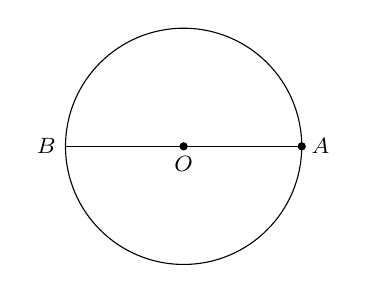
\begin{tikzpicture}[line join = round, line cap = round,>=stealth,font=\footnotesize,scale=1] 
	\def\R{1.5}
	\coordinate[label = below:$O$] (O) at (0,0); 
	\coordinate[label = right:$A$] (A) at (\R,0); 
	\draw (A)--++(-2*\R,0) node[left]{$B$}; 
	\draw (O) circle (\R);
	\foreach \x in {A,O} \fill[black] (\x) circle (1.5pt); 
\end{tikzpicture}
}
\end{note}
\subsubsection{Tính đối xứng của đường tròn}
\begin{boxdn}
 \begin{itemize}
 \item Đường tròn là hình có tâm đối xứng; tâm của đường tròn là tâm đối xứng của nó.
 \item Đường tròn là hình có trục đối xứng; mỗi đường thẳng đi qua tâm của đường tròn là một trục đối xứng của nó.
 \end{itemize}
\end{boxdn}
\begin{note}
 Đường tròn có một tâm đối xứng nhưng có vô số trục đối xứng.
\end{note}
%%%
	\subsubsection{Dây và đường kính của đường tròn}
\begin{boxdn}
	\noindent
	\begin{itemize}
	\item	Đoạn thẳng nối hai điểm tùy ý của một đường tròn gọi là một dây (hay dây cung) của đường tròn.
	\item	Mỗi dây đi qua tâm là một đường kính của đường tròn. Dễ thấy đường kính của đường tròn bán kính $R$ có độ dài bằng $2R$.
	\end{itemize}	
\end{boxdn}
\begin{boxdl}
	Trong một đường tròn, đường kính là dây cung lớn nhất.
\end{boxdl}
\subsubsection{Hai đường tròn cắt nhau}
\immini{
	\begin{boxdn}
	Nếu hai đường tròn có đúng hai điểm chung thì ta nói đó là hai đường tròn cắt nhau. Hai điểm chung đó gọi là hai giao điểm của chúng.
	\end{boxdn}
	\begin{nx}
	Hai đường tròn $\left(O;R\right)$ và $\left(O';R'\right)$ cắt nhau khi
	\begin{center}
	$R-R'<OO'<R+R'$ $\left(\text{với} \, R>R'\right)$.
	\end{center}
	\end{nx} 
}{
	\begin{tikzpicture}[line join = round, line cap = round,>=stealth,font=\footnotesize,scale=1] 
	\coordinate[label = left:$O$] (O) at (0,0); 
	\def\R{1.75}
	\def\r{1.25}
	\pgfmathsetmacro{\d}{\R+\r-1} 
	\coordinate[label = right:$O'$] (O') at (\d,0); 
	\draw[name path=dt1] (O) circle (\R) ;
	\draw[name path=dt2] (O') circle (\r);
	\path[name intersections={of= dt1 and dt2}] coordinate[label = above:$A$] (A) at (intersection-1) coordinate[label = below:$B$] (B) at (intersection-2); 
	\draw (O)--(O');
	\foreach \x in {O',O,A,B} \fill[black] (\x) circle (1.5pt); 
	\end{tikzpicture}
}
\subsubsection{Hai đường tròn tiếp xúc nhau}
\begin{boxdn}
	Nếu hai đường tròn có duy nhất một điểm chung thì ta nói đó là hai đường tròn tiếp xúc nhau. Điểm chung gọi là tiếp điểm của chúng.
\end{boxdn}
\begin{note}
	Người ta phân biệt hai trường hợp: hai đường tròn tiếp xúc ngoài (Hình a) và hai đường tròn tiếp xúc trong (Hình b).
\end{note}
\begin{center}
	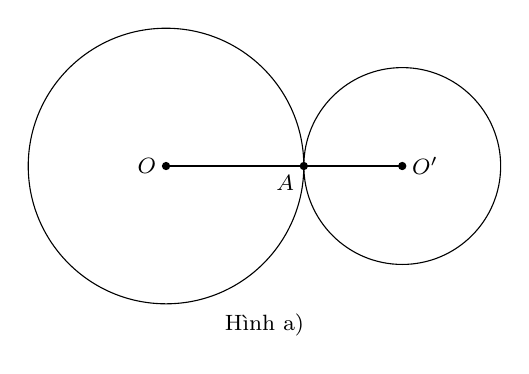
\begin{tikzpicture}[line join = round, line cap = round,>=stealth,font=\footnotesize,scale=1] 
	\coordinate[label = left:$O$] (O) at (0,0); 
	\def\R{1.75}
	\def\r{1.25}
	\pgfmathsetmacro{\d}{\R+\r} 
	\coordinate[label = right:$O'$] (O') at (\d,0); 
	\coordinate[label = below left:$A$] (A) at (\R,0);
	\draw (O) circle (\R) ;
	\draw (O') circle (\r);
	\draw (O)--(O');
	\foreach \x in {O',O,A} \fill[black] (\x) circle (1.5pt); 
	\path (current bounding box.south) node[below, black]{Hình a)};
	\end{tikzpicture}
	\hspace*{1cm}
	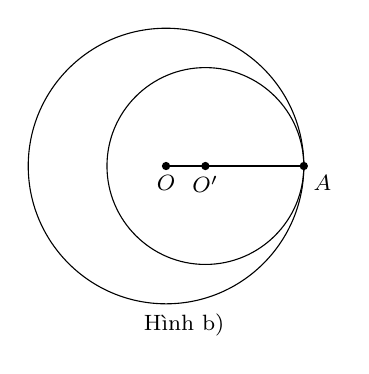
\begin{tikzpicture}[line join = round, line cap = round,>=stealth,font=\footnotesize,scale=1] 
	\coordinate[label = below:$O$] (O) at (0,0); 
	\def\R{1.75}
	\def\r{1.25}
	\pgfmathsetmacro{\d}{\R-\r} 
	\coordinate[label = below:$O'$] (O') at (\d,0); 
	\coordinate[label = below right:$A$] (A) at (\R,0);
	\draw (O) circle (\R) ;
	\draw (O') circle (\r);
	\draw (O)--(A);
	\foreach \x in {O',O,A} \fill[black] (\x) circle (1.5pt); 
	\path (current bounding box.south) node[below, black]{Hình b)};
	\end{tikzpicture}	
\end{center}
\begin{nx}
	\begin{itemize}
	\item Hai đường tròn $\left(O;R\right)$ và $\left(O';R'\right)$ tiếp xúc ngoài khi $OO'=R+R'$ và tiếp xúc trong khi $OO'=R-R'$ $\left(\text{với} \, R>R'\right)$.
	\item Nếu hai đường tròn tiếp xúc với nhau thì tiếp điểm thẳng hàng với hai tâm.
	\end{itemize}
\end{nx} 
\subsubsection{Hai đường tròn không giao nhau}
\begin{boxdn}
	Nếu hai đường tròn không có điểm chung nào thì ta nói đó là hai đường tròn không giao nhau.
\end{boxdn}
\begin{note}
	Người ta phân biệt hai trường hợp: hai đường tròn ngoài nhau (Hình a) và đường tròn này đựng đường tròn kia (Hình b).	
\end{note}
\begin{center}
	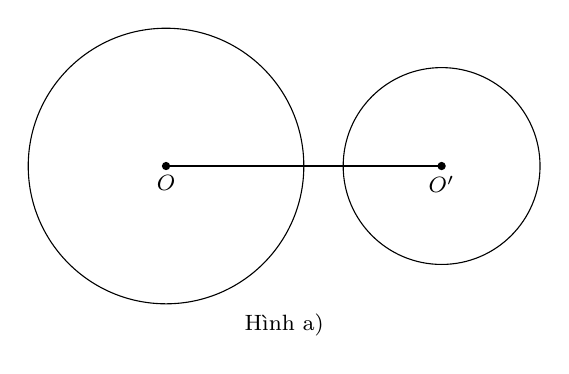
\begin{tikzpicture}[line join = round, line cap = round,>=stealth,font=\footnotesize,scale=1] 
	\coordinate[label = below:$O$] (O) at (0,0); 
	\def\R{1.75}
	\def\r{1.25}
	\pgfmathsetmacro{\d}{\R+\r+0.5} 
	\coordinate[label = below:$O'$] (O') at (\d,0); 
	\draw (O) circle (\R) ;
	\draw (O') circle (\r);
	\draw (O)--(O');
	\foreach \x in {O',O} \fill[black] (\x) circle (1.5pt); 
	\path (current bounding box.south) node[below, black]{Hình a)};
	\end{tikzpicture}
	\hspace*{1cm}
	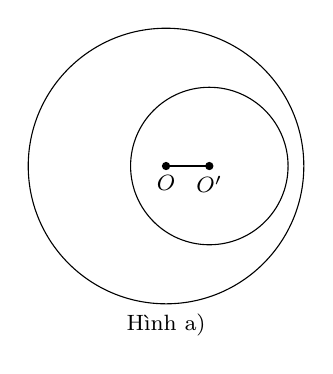
\begin{tikzpicture}[line join = round, line cap = round,>=stealth,font=\footnotesize,scale=1] 
	\coordinate[label = below:$O$] (O) at (0,0); 
	\def\R{1.75}
	\def\r{1}
	\pgfmathsetmacro{\d}{\R-\r-0.2} 
	\coordinate[label = below:$O'$] (O') at (\d,0); 
	\draw (O) circle (\R) ;
	\draw (O') circle (\r);
	\draw (O)--(O');
	\foreach \x in {O',O} \fill[black] (\x) circle (1.5pt); 
	\path (current bounding box.south) node[below, black]{Hình a)};
	\end{tikzpicture}
\end{center}
\begin{nx}
	\begin{itemize}
	\item Hai đường tròn $\left(O;R\right)$ và $\left(O';R'\right)$ ngoài nhau khi $OO'>R+R'$.
	\item Đường tròn $\left(O;R\right)$ đựng đường tròn $\left(O';R'\right)$ khi $R>R'$ và $OO'<R-R'$. Đặc biệt khi $O$ trùng với $O'$ và $R \neq R'$ thì ta có hai đường tròn đồng tâm.
	\end{itemize}
\end{nx} 
\subsubsection*{Ta có bảng tổng kết sau}
\begin{center}
	\begin{tabular}{|l|c|c|}
	\hline
	Vị trí tương đối của$\left(O;R \right)$ và $\left(O;R' \right)$ $\left(R \geq R'\right)$	&Số điểm chung&Hệ thức giữa $OO'$ với $R$ và $R'$\\ 
	\hline
	$\left(O \right)$ và $\left(O' \right)$ cắt nhau
	&$2$
	&$R-R'<OO'<R+R'$\\ 
	\hline
	$\left(O \right)$ và $\left(O' \right)$ tiếp xúc ngoài
	&$1$
	&$OO'=R+R'$\\
	\hline
	$\left(O \right)$ và $\left(O' \right)$ tiếp xúc trong
	&$1$
	&$OO'=R-R'>0$\\
	\hline
	$\left(O \right)$ và $\left(O' \right)$ ở ngoài nhau
	&$0$
	&$OO'>R+R'$\\
	\hline
	$\left(O \right)$ đựng $\left(O' \right)$
	&$0$
	&$OO'<R-R'$\\
	\hline
	\end{tabular}
\end{center}
\end{tomtat}
%%%%%%%%%%%%%%%%%%%
\subsection{Các dạng bài tập}
\begin{dang}{Chứng minh nhiều điểm cùng nằm trên một đường tròn}
\end{dang}
\begin{vd}%[9H2B1]
	Cho hình chữ nhật $ABCD$ có $AB=a$, $BC=b$. Chứng minh rằng bốn điểm $A$, $B$, $C$, $D$ cùng thuộc một đường tròn. Xác định tâm và tính bán kính của đường tròn đó.
	\loigiai{
	\immini{
	Gọi $O$ là giao điểm của hai đường chéo $AC$ và $BD$. Theo tính chất hai đường chéo của hình chữ nhật, ta có
	$OA=OB=OC=OD\left(=\dfrac{1}{2}AC=\dfrac{1}{2}BD\right).$\\
	Vậy bốn điểm $A$, $B$, $C$, $D$ cùng thuộc $\left(O;\dfrac{1}{2}AC\right)$.\\
	Áp dụng định lí Py-ta-go vào tam giác vuông $ABC$, ta có
	$$AC^2 =AB^2+BC^2 =a^2 +b^2.$$
	Do đó $R=\dfrac{1}{2}AC=\dfrac{1}{2}\sqrt{a^2+b^2}$.
	}{
	\begin{tikzpicture}[line join = round, line cap = round,>=stealth,
	font=\footnotesize,scale=0.8]
	\tkzDefPoints{0/0/D}
	\coordinate (C) at ($(D)+(5,0)$);
	\coordinate (A) at ($(D)+(0,3)$);
	\coordinate (B) at ($(A)+(C)-(D)$);
	\tkzInterLL(A,C)(B,D)
	\tkzGetPoint{O}
	\tkzDrawCircle[radius](O,A)
	%\pgfresetboundingbox
	\tkzDrawPolygon(A,B,C,D)
	\tkzDrawSegments(C,A B,D)
	\tkzMarkSegments[mark=|](A,O O,B O,C O,D)
	\tkzDrawPoints[fill=black](A,B,C,D,O)
	\tkzMarkRightAngles[size=0.2](A,B,C B,C,D C,D,A D,A,B)
	\tkzLabelPoints[above left](A)
	\tkzLabelPoints[above right](B)
	\tkzLabelPoints[below](O)
	\tkzLabelPoints[below left](D)
	\tkzLabelPoints[below right](C)
	\path (B)--(A) node[above,midway,sloped]{$a$};
	\path (B)--(C) node[above,midway,sloped]{$b$};
	\end{tikzpicture}	
	}
	}
\end{vd}
\begin{vd}%[9H2K1]
	Cho tam giác $ABC$, các đường cao $BD$ và $CE$. Trên cạnh $AC$ lấy điểm $M$. Kẻ tia $Cx$ vuông góc với tia $BM$ tại $F$. Chứng minh rằng năm điểm $B$, $C$, $D$, $E$, $F$ cùng thuộc một đường tròn.
	\loigiai{
	\immini{
	Gọi $O$ là trung điểm của $BC$. Ta có $BD$ là đường cao nên $BD\perp AC$, hay tam giác $BDC$ vuông tại $D$.\\
	Trong tam giác vuông $BDC$ có $DO$ là trung tuyến ứng với cạnh huyền $BC$ nên
	\begin{align*}
	OD=OB=OC=\dfrac{1}{2}BC\tag{1}
	\end{align*}
	Tương tự, ta có $OE=OB=OC=\dfrac{1}{2}BC$.\hfill$(2)$\\
	và $OF=OB=OC=\dfrac{1}{2}BC$.\hfill$(3)$\\
	Từ $(1)$, $(2)$ và $(3)$ suy ra $OB=OC=OD=OE=OF$.\\
	Do đó năm điểm $B$, $C$, $D$, $E$, $F$ cùng thuộc đường tròn $(O;R)$ với $R=\dfrac{1}{2}BC$. 
	}{
	\begin{tikzpicture}[line join = round, line cap = round,>=stealth,
	font=\footnotesize,scale=.7]
	\clip (-1,-4)rectangle(7,5);
	\tkzDefPoints{0/0/B}
	\coordinate (C) at ($(B)+(6,0)$);
	\tkzDefShiftPoint[B](75:4){A}
	\coordinate (O) at ($(C)!0.5!(B)$);
	\tkzDefPointBy[projection= onto A--C](B)
	\tkzGetPoint{D}
	\tkzDefPointBy[projection= onto A--B](C)
	\tkzGetPoint{E}
	\tkzDrawCircle[radius](O,B)
	\coordinate (M) at ($(C)!0.4!(D)$);
	\tkzDefPointBy[projection= onto B--M](C)
	\tkzGetPoint{F}
	\coordinate (x) at ($(C)!2.5!(F)$);
	%
	%\pgfresetboundingbox
	\tkzDrawSegments(A,B B,C C,A C,E B,D C,x B,F)
	\tkzMarkRightAngles[size=.2](C,E,B B,D,C B,F,C)
	\tkzDrawSegments[dashed](O,D O,E O,F)
	\tkzDrawPoints[fill=black](A,B,C,O,D,E,M,F)
	\tkzLabelPoints[above](A,D,x,M)
	\tkzLabelPoints[left](B,E)
	\tkzLabelPoints[right](C,F)
	\tkzLabelPoints[below](O)
	\end{tikzpicture}	
	}
	}
\end{vd}
\begin{vd}%[9H2K1]
	Chứng minh rằng bốn trung điểm của bốn cạnh hình thoi cùng thuộc một đường tròn.
	\loigiai{
	\immini{
	Gọi $M$, $N$, $P$, $Q$ lần lượt là trung điểm của bốn cạnh $AB$, $BC$, $CD$ và $DA$ của hình thoi $ABCD$.
	Gọi $O$ là giao điểm của $AC$ và $BD$. Ta có $AC\perp BD$. Theo tính chất đường trung tuyến ứng với cạnh huyền của tam giác vuông, ta được $OM=\dfrac{1}{2}AB$; $ON=\dfrac{1}{2}BC$; $OP=\dfrac{1}{2}CD$; $OQ=\dfrac{1}{2}AD$.\\
	Mặt khác $AB=BC=CD=DA$ nên $OM=ON=OP=OQ$. Do đó bốn điểm $M$, $N$, $P$, $Q$ cùng nằm trên một đường tròn.
	}{
	\begin{tikzpicture}[line join = round, line cap = round,>=stealth,
	font=\footnotesize,scale=.7]
	\tkzDefPoints{0/0/A}
	\def \gocA{50}; %sŁ đo góc A
	\def \canh{5}; %đº dài c⁄nh
	\tkzDefShiftPoint[A](\gocA/2:\canh){B}
	\tkzDefShiftPoint[A](-\gocA/2:\canh){D}
	\coordinate (C) at ($(B)+(D)-(A)$);
	\tkzInterLL(A,C)(B,D)
	\tkzGetPoint{O}
	\coordinate (M) at ($(A)!0.5!(B)$);
	\coordinate (N) at ($(C)!0.5!(B)$);
	\coordinate (P) at ($(C)!0.5!(D)$);
	\coordinate (Q) at ($(A)!0.5!(D)$);
	\tkzDrawCircle[radius](O,M)
	%
	\pgfresetboundingbox
	\tkzDrawPolygon(A,B,C,D)
	\tkzDrawPoints[fill=black](A,B,D,C,O,M,N,P,Q)
	\tkzDrawSegments(A,C B,D)
	\tkzDrawSegments[dashed](M,P N,Q)
	\tkzLabelPoints[above](B)
	\tkzLabelPoints[below](D)
	\tkzLabelPoints[left](A)
	\tkzLabelPoints[right](C)
	\tkzLabelPoints[above left](M)
	\tkzLabelPoints[above right](N)
	\tkzLabelPoints[below left](Q,O)
	\tkzLabelPoints[below right](P)
	\end{tikzpicture}	
	}
	}
\end{vd}
%================
\begin{dang}{Xác định vị trí tương đối của điểm $M$ với đường tròn $(O)$}
%	Tính khoảng cách $OM=d$. Khi đó
%	\begin{itemize}
%	\item $d>R\Leftrightarrow M$ nằm ngoài $(O;R)$.
%	\item $d=R\Leftrightarrow M$ nằm trên $(O;R)$.
%	\item $d<R\Leftrightarrow M$ nằm trong $(O;R)$.
%	\end{itemize}
\end{dang}
\begin{vd}
	\immini{
	Gọi $O$ là trung điểm của đoạn thẳng $AB$. Chứng minh rằng đường tròn $(O;OA)$ đi qua điểm $B$.
	}{
	\begin{tikzpicture}[scale=0.65,line cap=round,line join=round,>=triangle 45,x=1.0cm,y=1.0cm]
	\coordinate (tam) at (0,0);
	\coordinate (A) at (180:2);
	\coordinate (B) at (0:2);
	\def\bankinh{2}
	\draw (tam) circle [radius=\bankinh];
	\draw (A)--(B);
	\draw ($(tam)!1/2!(A)$) node[scale=0.8,above] {$R$};
	\fill (tam) circle[radius=1.5pt] node[scale=0.8,below] {O}
	(A) circle[radius=1.5pt] node[scale=0.8,left] {A}
	(B) circle[radius=1.5pt] node[scale=0.8,right] {B}
	;
	\end{tikzpicture}
	}
	\loigiai{
	Vì $O$ là trung điểm của $AB$ nên $OA=OB$.\\
	Do đó $B \in (O;OA)$, nói cách khác, đường tròn $(O;OA)$ đi qua điểm $B$.
	}
\end{vd}
\begin{vd}
	Cho tam giác $ABC$ vuông tại $A$. Chứng minh rằng điểm $A$ thuộc đường tròn đường kính $BC$.
	\loigiai{
	\immini{
	Gọi $O$ là trung điểm của $BC$.\\
	Theo tính chất trung tuyến ứng với cạnh huyền bằng nửa cạnh huyền, do đó $OA=OB=OC$.\\
	Vậy $A \in (O;OB)$, nói cách khác, $A$ thuộc đường tròn đường kính $BC$.
	}{
	\begin{tikzpicture}[line cap=round,line join=round,>=triangle 45,x=1.0cm,y=1.0cm,scale=0.7]
	\path 
	(0,0) coordinate (O) 
	(120:2) coordinate (A)
	(180:2) coordinate (B)
	(0:2) coordinate (C)
	;
	\def\bankinh{2}
	\draw (O) circle [radius=\bankinh];
	\draw (A)--(B)--(C)--(A)--(O);
	\draw pic[draw,angle radius=2mm]{right angle=B--A--C};
	\foreach \p/\g in {A/90,B/-140,C/-30,O/-90} 
	\fill (\p) circle(1.5pt) node [scale=0.8,shift={(\g:.3)}] {$\p$}; 
	\end{tikzpicture}
	}
	}
\end{vd}
\begin{vd}
	Trong mặt phẳng tọa độ $Oxy$, cho các điểm $A(3;0)$, $B(-2;0)$, $C(0;4)$. Vẽ hình và cho biết trong các điểm đã cho, điểm nào nằm trên, điểm nào nằm trong, điểm nào nằm ngoài đường tròn $(O;3)$?
	\loigiai{
	\immini{
	Dựa vào hình vẽ ta thấy
	\begin{itemize}
	\item Điểm $A$ nằm trên đường tròn $(O;3)$.
	\item Điểm $B$ nằm trong đường tròn $(O;3)$.
	\item Điểm $C$ nằm ngoài đường tròn $(O;3)$.
	\end{itemize}
	}{
	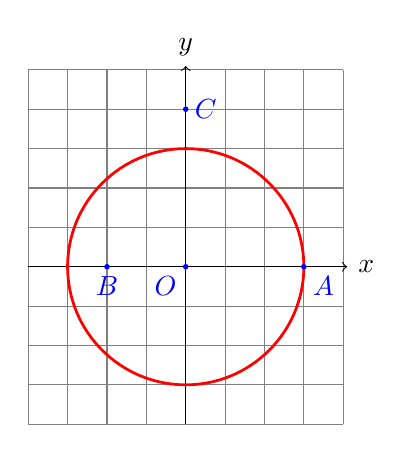
\begin{tikzpicture}[scale=0.5,every node/.style={minimum size=0.5cm-\pgflinewidth, outer sep=0pt}]
	\draw[step=1cm,color=gray] (-4,-4) grid (4,5);
	\draw[->] (-4,0)--(4.1,0) node[right] {$x$};
	\draw[->] (0,-4)--(0,5.1) node[above] {$y$};
	\coordinate (tam) at (0,0);
	\coordinate (B) at (-2,0);
	\coordinate (C) at (0,4);
	\coordinate (A) at (3,0);
	\def\bankinh{3}
	\draw[red,line width=1pt] (tam) circle [radius=\bankinh];
	\fill[blue] (tam) circle[radius=2pt] node[below left] {$O$}
	(B) circle[radius=2pt] node[below] {$B$}
	(C) circle[radius=2pt] node[right] {$C$}
	(A) circle[radius=2pt] node[below right] {$A$}
	;
	\end{tikzpicture}
	}
	}
\end{vd}
\begin{vd}
	\immini{
	Cho đường tròn $(O; R)$ và năm điểm $M$; $N$; $P$; $H$; $K$. So sánh độ dài các đoạn thẳng $OM$; $ON$; $OH$; $OK$; $OP$ với $R$.
	}{
	\begin{tikzpicture}[scale=1, font=\footnotesize, line join=round, line cap=round, >=stealth]
	\def\r{1.5}	
	\path (0,0) coordinate (O)
	($(O)+(20:\r)$) coordinate (H)
	($(O)+(20:1.5*\r)$) coordinate (P)
	($(O)+(60:\r)$) coordinate (M)
	($(O)+(-60:\r)$) coordinate (K)
	($(O)+(-60:0.4*\r)$) coordinate (N);
	\pgfresetboundingbox
	\draw (O) let \p1=($(O)-(H)$) in circle ({veclen(\x1,\y1)});
	\draw (O)--(P) (O)--(M) (O)--(K);
	\foreach \x/\g in {O/180,K/-90,H/70,N/0,M/90,P/0}\draw[fill=black](\x) circle (.05) + (\g:.4) node{$\x$};
	\end{tikzpicture}
	}
	\loigiai{Vì $M, H, K$ thuộc $(O ; R)$ nên $O M=O H=O K=R$.
	Ta có: $O N<O K$ nên $O N<R$; $O P>O H$ nên $O P>R$.}
\end{vd}
\begin{vd}%[9H2B1]
	Cho đường tròn $(O;R)$ và hai điểm $M$, $N$ sao cho $M$ nằm trong và $N$ nằm ngoài $(O;R)$. Hãy so sánh $\widehat{OMN}$ và $\widehat{ONM}$.
	\loigiai{
	\immini{
	Ta có $M$ nằm trong $(O;R)$ nên $OM<R$, $N$ nằm ngoài $(O;R)$ nên $ON>R$.\\
	Trong tam giác $OMN$, có $OM<ON$ (vì
	$OM<R$, $ON>R$) nên $\widehat{OMN}>\widehat{ONM}$ (trong một tam giác, góc đối diện với cạnh lớn hơn thì lớn hơn).
	}{
	\begin{tikzpicture}[line join = round, line cap = round,>=stealth,
	font=\footnotesize,scale=0.5]
	\tkzDefPoints{0/0/O,-1.5/2/M,5/2.2/N}
	\draw (O) circle (3cm);
	\tkzDrawPoints[fill=black](O,M,N)
	\tkzDrawSegments(O,M O,N M,N)
	\tkzMarkAngles[size=1,arc=l](O,M,N)
	\tkzMarkAngles[size=1.5,arc=ll](M,N,O)
	\tkzLabelPoints[below](O)
	\tkzLabelPoints[below left](M)
	\tkzLabelPoints[right](N)
	\end{tikzpicture}	
	}
	}
\end{vd}
%=================
\begin{dang}{Tâm đối xứng, trục đối xứng của đường tròn}
\end{dang}
\begin{vd}
	\immini{Xác định tâm đối xứng và trục đối xứng của bánh xe trong hình bên.}{
	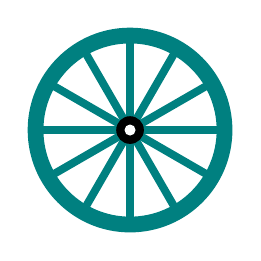
\begin{tikzpicture}[>=stealth,line join=round,line cap=round,font=\footnotesize,scale=1]
	\def\R{1.2}
	\draw[teal,line width=2mm] (0,0) circle (\R cm);
	\foreach \i in {1,...,12}{
	\draw[teal,line width=1mm] (0,0)--(\i*30:\R);	
	}
	\fill circle (5pt);
	\fill[white] circle (2pt);
	\end{tikzpicture}
	}
	\loigiai{
	Tâm đối xứng trong Hình $7$ là giao điểm các đường thẳng đi qua tâm.\\
	Trục đối xứng là các đường thẳng đi qua tâm.
	}
\end{vd}
\begin{vd}
	\immini{
	Nêu cách chia một cái bánh có dạng hình tròn tâm $O$ (Hình bên) thành hai phần bằng nhau.}{
	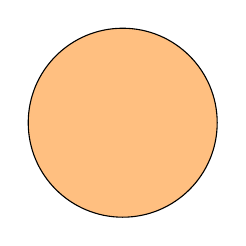
\begin{tikzpicture}[>=stealth,line join=round,line cap=round,font=\footnotesize,scale=1]
	\def\R{1.2}
	\draw[fill=orange!50] (0,0) circle (\R cm);
	\end{tikzpicture}
	}
	\loigiai{
	Vẽ đường thẳng đi qua tâm khi đó đường thẳng sẽ chia cái bánh thành 2 phần bằng nhau.
	}
\end{vd}
\begin{vd}
	Cho đường tròn $(I)$.
	\begin{listEX} [2]
	\item Tìm tâm đối xứng của $(I)$;
	\item Vẽ hai trục đối xứng của $(I)$.
	\end{listEX} 
	\loigiai{
	\immini{\begin{enumerate}[a)]
	\item Tâm $I$ là tâm đối xứng của $(I)$.
	\item Vẽ hai đường thẳng $a$ và $b$ đi qua tâm $I$. Ta có $a$ và $b$ đều là trục đối xứng của $(I)$.
	\end{enumerate}}{	
	\begin{tikzpicture}
	\def\r{1.2}
	\path
	(0,0) coordinate (I)
	(15:2) coordinate (B)
	(195:2) coordinate (B')
	(-15:2) coordinate (A)
	(165:2) coordinate (A');
	\coordinate (J) at ($(A')!-1/6!(A)$);
	\coordinate (K) at ($(A')!7/6!(A)$);
	\coordinate (P) at ($(B')!-1/6!(B)$);
	\coordinate (Q) at ($(B')!7/6!(B)$);
	\draw (I) circle (\r);
	\draw [samples=200,smooth,red,line width=1](P)--(B')--(I)--(B)--(Q)--cycle node[below]{$b$};
	\draw [samples=200,smooth,red,line width=1](J)--(A')--(I)--(A)--(K)--cycle node[below]{$a$};
	\foreach \p/\r in {I/-90}
	\fill (\p) circle (1.5pt) node[shift={(\r:3mm)}]{$\p$};
	\end{tikzpicture}}
	}
\end{vd}
\begin{vd}
	Bạn Oanh có một mảnh giấy hình tròn nhưng không còn dấu vết của tâm. Theo em, Oanh làm thế nào để tìm lại được tâm của mảnh giấy hình tròn đó?
	\loigiai{
	Bằng cách gấp đôi mảnh giấy hình tròn theo hai cách khác nhau, Oanh có thể tìm lại được tâm của mảnh giấy hình tròn đó.
	}
\end{vd}
\begin{vd}
	Cho điểm $M$ nằm trên đường tròn $(O)$ đường kính $AB$. Sử dụng tính đối xứng của đường tròn $(O)$, hãy nêu cách tìm
	\begin{enumerate}
	\item Điểm $N$ đối xứng với điểm $M$ qua tâm $O$;
	\item Điểm $P$ đối xứng với điểm $M$ qua đường thẳng $AB$.
	\end{enumerate}
	\loigiai{
	\immini{
	\begin{enumerate}
	\item Do $O$ là tâm đối xứng của $(O)$ nên điểm $N$ đối xứng với điểm $M$ qua tâm $O$ phải vừa thuộc $OM$, vừa thuộc $(O)$. Vậy $N$ là giao điểm của đường thẳng $OM$ với $(O)$.
	\item Do $AB$ là trục đối xứng của $(O)$ nên điểm $P$ đối xứng với điểm $M$ qua $AB$ phải vừa thuộc $(O)$, vừa thuộc đường thẳng vuông góc hạ từ $M$ xuống $AB$. Vậy $P$ là giao điểm của $(O)$ với đường thẳng đi qua $M$ và vuông góc với $AB$.
	\end{enumerate}
	}{
	\begin{tikzpicture}[scale=0.8, font=\footnotesize, line join=round, line cap=round, >=stealth]
	\path 
	(0,0) coordinate (O) 
	(180:2) coordinate (A) 
	(0:2) coordinate (B)
	(180:2.5) coordinate (A') 
	(0:2.5) coordinate (B') 
	(60:2) coordinate (M)
	(60:2.5) coordinate (M')
	(240:2) coordinate (N)
	(240:2.5) coordinate (N')
	($(A)!(M)!(B)$) coordinate (H)
	($(M)!2!(H)$) coordinate (P)
	($(H)!1.3!(M)$) coordinate (E)
	($(H)!1.3!(P)$) coordinate (E')
	;
	\def\bankinh{2}
	\draw (O) circle [radius=\bankinh];
	\draw (A')--(B') (M')--(N') (E)--(E');
	\draw pic[draw,angle radius=2mm]{right angle=M--H--O};
	\foreach \p/\g in {A/-130,B/-40,M/20,N/-70,O/100,H/-50,P/-50} 
	\fill (\p) circle(1.5pt) node [scale=0.8,shift={(\g:.3)}] {$\p$}; 
	\end{tikzpicture}
	}
	}
\end{vd}
\begin{vd}
	Cho đường tròn tâm $O$ và hai điểm $A,B$ thuộc $(O)$. Gọi $d$ là đường trung trực của đoạn $AB$. Chứng minh rằng $d$ là một trục đối xứng của $(O)$.
	\loigiai{
	\immini{
	Do $A,B$ thuộc $(O)$ nên $OA=OB \Rightarrow O \in d$.\\
	Vậy $d$ là đường thẳng đi qua tâm $O$ của $(O)$, do đó $d$ là một trục đối xứng của $(O)$.
	}{
	\begin{tikzpicture}[scale=0.8, font=\footnotesize, line join=round, line cap=round, >=stealth]
	\path 
	(0,0) coordinate (O) 
	(180:2.5) coordinate (A') 
	(0:2.5) coordinate (B') 
	(60:2) coordinate (A)
	($(A')!(A)!(B')$) coordinate (H)
	($(A)!2!(H)$) coordinate (B)
	;
	\def\bankinh{2}
	\draw (O) circle [radius=\bankinh];
	\draw (A')--(B') node[below] {$d$} (A)--(O)--(B)--(A);
	\foreach \p/\g in {A/50,B/-50,O/-110} 
	\fill (\p) circle(1.5pt) node [scale=0.8,shift={(\g:.3)}] {$\p$}; 
	\end{tikzpicture}
	}
	}
\end{vd}
%==================
%%==========Ví dụ 1
\begin{vd}
	Cho tam giác nhọn $A B C$. Đường tròn tâm $O$ đường kính $B C$ cắt các canh $A B$ và $A C$ lần lượt tại $M$ và $N$. Chứng minh $MN<BC$.
	\loigiai{
	\immini{
	Xét $(O)$ có $BC$ là dây đường kính.\\
	Suy ra $BC$ là dây lớn nhất của đường tròn.\\
	Suy ra $MN < BC$.
	}{
	\begin{tikzpicture}[scale=0.5, font=\footnotesize, line join=round, line cap=round, >=stealth]
	\path (0,0) coordinate (B)
	(1,3) coordinate (A)
	(6,0) coordinate (C)
	($(B)!0.5!(C)$) coordinate (O);
	\path[name path = dtO](O) let \p1=($(O)-(B)$) in circle ({veclen(\x1,\y1)});	
	\path[name path = dtAB] (A)--(B);
	\path[name path = dtAC] (A)--(C);
	\path[name intersections = {of = dtO and dtAB, by ={M}}];
	\path[name intersections = {of = dtO and dtAC, by ={C,N}}];
	\pgfresetboundingbox
	\draw (A)--(B)--(C)--(A) (M)--(N);
	\draw[red](O) let \p1=($(O)-(B)$) in circle ({veclen(\x1,\y1)});
	\foreach \x/\g in {A/90,O/-90,C/0,B/180,M/180,N/90}\draw[fill=black](\x) circle (.05) + (\g:.4) node{$\x$};
	\end{tikzpicture}
	}
	}
\end{vd}
%%==========Ví dụ 2
\begin{vd}
	\immini{Bạn Mai căng ba đoạn chỉ $AB$, $CD$, $EF$ có độ dài lần lượt là $16$ cm, $14$ cm và $20$ cm trên một khung thêu hình tròn bán kính $10$ cm. Trong ba dây trên, dây nào đi qua tâm của đường tròn?}{
	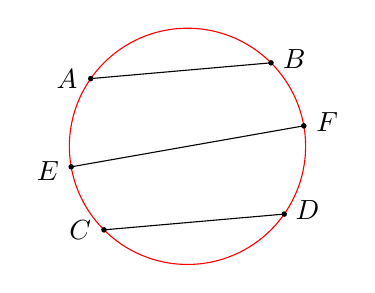
\begin{tikzpicture}
	\def\R{1.5}
	\path
	(0,0) coordinate (I)
	(10:\R) coordinate (F)
	(190:\R) coordinate (E)
	(45:\R) coordinate (B)
	(145:\R) coordinate (A)
	(-35:\R) coordinate (D)
	(-135:\R) coordinate (C);
	\draw [red] (I) circle (\R);
	\draw (E)--(I)--(F)--cycle;
	\draw (C)--(D);
	\draw (A)--(B);
	\foreach \p/\r in{A/180,B/10,D/10,C/180,F/10,E/190}
	\fill (\p) circle (1pt) node[shift={(\r:3mm)}]{$\p$};
	\end{tikzpicture}
	}
	\loigiai{Do $AB<EF$, $CD<EF, EF=2R$ nên trong 3 dây trên, dây đi qua tâm của đường tròn là dây $EF$.
	}
\end{vd}
%%==========Ví dụ 3
\begin{vd}
	\immini{Cho đường tròn $(I)$ có các dây cung $AB$, $CD$, $EF$. Cho biết $AB$ và $CD$ đi qua tâm $I$, $EF$ không đi qua $I$. Hãy so sánh độ dài $AB$, $CD$, $EF$.}{	
	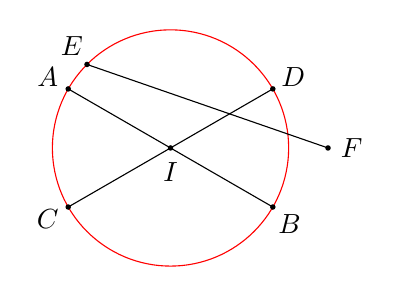
\begin{tikzpicture}
	\def\R{1.5}
	\path
	(0,0) coordinate (I)
	(-30:\R) coordinate (B)
	(150:\R) coordinate (A)
	(30:\R) coordinate (D)
	(210:\R) coordinate (C)
	(135:\R) coordinate (E)
	(0:2) coordinate (F);
	\draw[red] (I) circle (\R);
	\draw (A)--(I)--(B)--cycle;
	\draw (C)--(I)--(D)--cycle;
	\draw (E)--(F);
	\foreach \p/\r in {I/-90,A/150,B/-45,C/210,D/30,E/130,F/0}
	\fill (\p) circle (1pt) node[shift={(\r:3mm)}]{$\p$};
	\end{tikzpicture}
	}
	\loigiai{
	Ta có $AB$ là đường kính, $CD$ là đường kính, $EF$ là dây cung nên $AB=CD>EF$.
	}
\end{vd}
%%==========Ví dụ 4
\begin{vd}
	\immini{
	Trong hình bên, so sánh độ dài của các đoạn thẳng $OC$, $PQ$ với $AB$.
	}{
	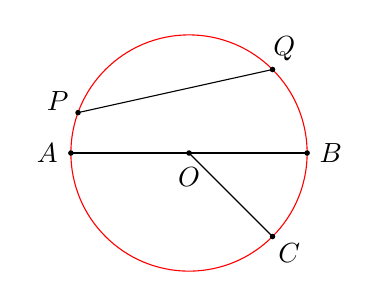
\begin{tikzpicture}
	\def\R{1.5}
	\path
	(0,0) coordinate (O)
	(-45:\R) coordinate (C)
	(45:\R) coordinate (Q)
	(160:\R) coordinate (P)
	(0:\R) coordinate (B)
	(180:\R) coordinate (A)
	;
	\draw[red] (O) circle (\R);
	\draw (A)--(O)--(B)--cycle;
	\draw (O)--(C);
	\draw (P)--(Q);
	\foreach \p/\r in {O/-90,A/180,B/0,Q/60,P/150,C/-45}
	\fill (\p) circle (1pt) node[shift={(\r:3mm)}]{$\p$};
	\end{tikzpicture}
	}
	\loigiai{
	Trong đường tròn $(O)$, $AB$ là đường kính, $OC$ là bán kính, $PQ$ là dây cung không đi qua $O$. Suy ra $OC=\dfrac{AB}{2}$ và $PQ<AB$.
	}
\end{vd}
%%==========Ví dụ 5
\begin{vd}
	Cho đường tròn đường kính $BC$. Chứng minh rằng với điểm $A$ bất kì (khác $B$ và $C$) nằm trên đường tròn, ta đều có $BC < AB+AC < 2 BC$. 
	\loigiai{
	\immini{	Áp dụng bất đẳng thức hình học cho $\triangle ABC$\\ ta luôn có $BC < AB + AC$.\hfill (1)\\
	Vì BC là đường kính của đường tròn nên\\
	$\left.\begin{aligned} AB < BC&\\ AC < BC&
	\end{aligned}\right. \Rightarrow AB+AC< 2BC$. \hfill \quad (2)\\
	Từ (1) và (2) ta suy ra $BC < AB+AC < 2 BC$ (đpcm).}
	{\begin{tikzpicture}[declare function={r=1.5;ga=120;gd=40;}]
	\path (0,0) coordinate (O) %tam
	(-180:r) coordinate (B)
	(0:r) coordinate (C)
	(ga:r) coordinate (A)	;
	\draw[red] (O) circle (r);
	\draw (A)--(B)--(C)--cycle;
	\foreach \t/\g in {A/120,B/180,C/0,O/-90}{
	\fill (\t) circle (1pt) node[shift={(\g:7pt)},font=\scriptsize]{$ \t $};	}
	\foreach \x/\y/\z in {B/A/C}{
	\path pic[draw,angle radius=5pt]{right angle= \x--\y--\z};	}
	\end{tikzpicture}}
	}
\end{vd}
%%==========Ví dụ 6
\begin{vd}
	Trong một trò chơi, hai bạn Thuỷ và Tiến cùng chạy trên một đường tròn tâm $O$ có bán kính $20$ m. Có thời điểm nào dây $AB$ nối vị trí của hai bạn đó có độ dài bằng $41$ m hay không? Vì sao?
	\begin{center}
	\begin{tikzpicture}[scale=1, font=\footnotesize, line join=round, line cap=round, >=stealth]
	\def\r{1.5}	
	\path (0,0) coordinate (O)
	($(O) + (150: \r)$) coordinate (A) node[left]{Thuỷ}
	($(O) + (30: \r)$) coordinate (B) node[right]{Tiến};
	\draw (O) let \p1=($(O)-(A)$) in circle ({veclen(\x1,\y1)});
	\draw (O)--(A)--(B)--(O);
	\foreach \x/\g in {O/-90,A/90,B/90}\draw[fill=black](\x) circle (1pt) + (\g:.4) node{$\x$};
	\end{tikzpicture}
	\end{center}
	\loigiai{
	Đường tròn tâm $O$ có đường kính là $2 \cdot 20=40$ m.\\
	Vì độ dài dây $AB$ không vượt quá độ dài đường kính của đường tròn nên $AB \leq 40$.\\
	Vậy không có thời điểm nào dây $AB$ nối vị trí của hai bạn đó có độ dài bằng $41$ m.	
	}
\end{vd}
%%==========Ví dụ 7
\begin{vd}
	Tứ giác lồi $ABCD$ có $\widehat{BAC}=\widehat{BDC}=90^{\circ}$. Chứng minh bốn điểm $A$, $B$, $C$, $D$ cùng nằm trên một đường tròn và $AD < BC$. 
	\loigiai{
	\immini{ Gọi $O$ là trung điểm của đoạn $BC$.\\ Tam giác $\triangle ABC$ vuông tại $A\left(\widehat{BAC}=90^{\circ}\right)$ nên đường trung tuyến $AO$ bằng nửa cạnh huyền.\\ Nghĩa là $OA=OB=OC=\dfrac{BC}{2}$.\\ Do đó điểm $A$ nằm trên đường tròn $(O)$ đường kính $BC$.\\
	Tương tự, bằng cách xét tam giác $\triangle DBC$ ta cũng suy ra điểm $D$ thuộc đường tròn $(O)$.\\ Vậy $AD$ là một dây (không đi qua tâm) của đường tròn $(O)$.\\ Áp dụng định lí trên ta có $AD < BC$. }
	{\begin{tikzpicture}[declare function={r=1.9;ga=120;gd=40;}]
	\path (0,0) coordinate (O) %tam
	(-180:r) coordinate (B)
	(0:r) coordinate (C)
	(ga:r) coordinate (A)
	(gd:r) coordinate (D);
	\draw[dashed,red] (O) circle (r);
	\draw (A)--(B)--(C)--(D)--cycle--(A)--(O)--(D)--(B) (A)--(C);
	\foreach \t/\g in {A/120,B/180,C/0,D/60,O/-90}{
	\fill (\t) circle (1pt) node[shift={(\g:7pt)},font=\scriptsize]{$ \t $};	}
	\foreach \x/\y/\z in {B/A/C,B/D/C}{
	\path pic[draw,angle radius=5pt]{right angle= \x--\y--\z};	}
	\end{tikzpicture}}
	}
\end{vd}
%%==========Ví dụ 8
\begin{vd}%[9H2B2]
	Cho đường tròn tâm $O$ bán kính $R=5$ cm, dây $AB=8$ cm. Gọi $I$ là điểm trên dây $AB$ sao cho $AI=1$ cm. Kẻ dây $CD$ đi qua điểm $I$ và vuông góc với dây $AB$. Chứng minh rằng $AB=CD$.
	\loigiai{
	\immini{
	Vẽ $OH\perp AB$, $OK\perp CD$. Suy ra $HA=HB=\dfrac{1}{2}AB=\dfrac{1}{2}\cdot8=4$ cm.\\
	Ta có $IH=AH-Al=4-1=3$ cm.\\
	Áp dụng định lí Py-ta-go vào tam giác vuông $HOB$. ta có
	$$OH^2=OB^2-HB^2=5^2-4^2=9\Rightarrow OH=3\text{ cm}.$$
	Suy ra tứ giác $OHIK$ là hình vuông. Do đó $OM=OK(=3\text{ cm})\Rightarrow AB=CD$.
	}{
	\begin{tikzpicture}[scale=0.4, font=\footnotesize, line join=round, line cap=round, >=stealth]
	\tikzset{label style/.style={font=\footnotesize}}
	\tkzDefPoints{0/0/O, 4/-3/B, -4/-3/A, -3/-3/I, -3/0/K}	
	\tkzDrawCircle[radius](O,A) 	
	\tkzInterLC(K,I)(O,A) \tkzGetPoints{D}{C}
	\coordinate (H) at ($(A)!0.5!(B)$);
	\coordinate (a) at ($(O)!0.5!(B)$);
	\draw[] (a) node[above] {$5$};
	\tkzDrawSegments(A,B O,B C,D O,K O,H)
	\tkzDrawPoints[fill=black](O,A,B,I,K,C,D,H)	
	\tkzLabelPoints[above](O,D)
	\tkzLabelPoints[right](B)
	\tkzLabelPoints[above left](I)
	\tkzLabelPoints[left](A,K)
	\tkzLabelPoints[below](C,H)
	\tkzMarkRightAngles[size=0.4,fill=gray!50](O,H,B O,K,I)
	\tkzMarkSegments[mark=||](K,D K,C)
	\tkzMarkSegments[mark=||](H,A H,B)
	\end{tikzpicture}
	}
	}
\end{vd}
%==================
\begin{dang}{Tính độ dài của một dây. Tính khoảng cách từ tâm đến dây}
\end{dang}
%%==========Ví dụ 24
\begin{vd}%[9H2B3]
	Cho đường tròn $(O;10)$. Lấy một điểm $A$ tùy ý thuộc $(O)$. Vẽ dây $MN$ vuông góc với $OA$ tại trung điểm của $OA$. Tính độ dài dây $MN$.
	\loigiai{
	\immini{
	Gọi $I$ là trung điểm của $OA$. Ta có $OI=\dfrac{1}{2}OA=\dfrac{1}{2}\cdot 10=5$.\\
	Áp dụng định lý Py-ta-go vào tam giác vuông $IMO$, ta được
	$$IM^2 =OM^2-OI^2=10^2-5^2=75 \Rightarrow IM=5\sqrt{3}$$
	Ta có $MN$ vuông góc $OA$ tại trung điểm $I$ của $OA$, nên
	$$IM=IN=\dfrac{1}{2}MN\Rightarrow MN=2IM=2\cdot5\sqrt{3}=10\sqrt{3}.$$
	}{
	\begin{tikzpicture}[scale=0.6, font=\footnotesize, line join=round, line cap=round, >=stealth]
	\tikzset{label style/.style={font=\footnotesize}}
	\tkzDefPoints{0/0/O,-3/0/A}
	\tkzDrawCircle[radius](O,A)
	\coordinate (I) at ($(A)!0.5!(O)$);
	\tkzDefLine[perpendicular=through I,K=.2](A,O) \tkzGetPoint{i} 
	\tkzInterLC(I,i)(O,A) \tkzGetPoints{M}{N}
	\coordinate (a) at ($(M)!0.5!(O)$);
	\draw (a) node[right] {$R$};
	\tkzDrawSegments(A,O M,N)
	\tkzDrawSegments[dashed](O,M)
	\tkzDrawPoints[fill=black](A,M,N,O,I)
	\tkzLabelPoints[above](M) 
	\tkzLabelPoints[left](A)
	\tkzLabelPoints[below left](I)
	\tkzLabelPoints[right](O) 
	\tkzLabelPoints[below](N)
	\tkzMarkRightAngles[size=.3,fill=gray!50](M,I,A) 
	\tkzMarkSegments[mark=||,size=0.1](A,I I,O)
	\end{tikzpicture}
	}
	}
\end{vd}
%%==========Ví dụ 25
\begin{vd}%[9H2B3]
	Cho đường tròn $(O;R)$ và dây $MN=R$. Hãy tính khoảng cách từ tâm $O$ đến dây $MN$.
	\loigiai{
	\immini{
	Vẽ $OH\perp MN$ tại $H$ thì $MH=HN=\dfrac{1}{2}MN=\dfrac{R}{2}$.\\
	Áp dụng định lí Py-ta-go vào tam giác $OMH$ có $OM^2=OH^2+MH^2$.
	\begin{eqnarray*}
	&\Rightarrow&OH^2=OM^2-MH^2=R^2-\left(\dfrac{R}{2}\right)^2 =\dfrac{3R^2}{4}\\
	&\Rightarrow&OH=\sqrt{\dfrac{3R^2}{4}}=\dfrac{R\sqrt{3}}{2}.
	\end{eqnarray*}
	Vậy khoảng cách từ tâm $O$ đến dây $MN$ là $\dfrac{R\sqrt{3}}{2}$.
	}{
	\begin{tikzpicture}[scale=1, font=\footnotesize, line join=round, line cap=round, >=stealth]
	\tikzset{label style/.style={font=\footnotesize}}
	\def\h{2}
	\pgfmathsetmacro\goc{70}
	\pgfmathsetmacro\xmin{-1.2*\h}
	\pgfmathsetmacro\xmax{1.5*\h}
	\pgfmathsetmacro\ymin{-1.3*\h}
	\pgfmathsetmacro\ymax{1.3*\h}
	\clip(\xmin-0.01,\ymin-0.01)rectangle(\xmax+0.01,\ymax+0.01);
	\tkzDefPoint(0,0){O}
	\tkzDefShiftPoint[O](0:\h){N}
	\coordinate (m) at ($(O)!1/2.236!(N)$);
	\tkzDefPointsBy[rotation = center O angle \goc](N,m){M,n}
	\coordinate (H) at ($(M)!1/2!(N)$);
	\tkzDrawSegments(O,N O,M N,M O,H)
	\draw (O) circle (\h);
	\tkzDrawPoints[fill=black](O,N,M,H)
	\tkzLabelPoints[left](O)
	\tkzLabelPoints[right](N)
	\draw[below](m)node{$R$};
	\draw[left](n)node{$R$};
	\tkzLabelPoints[above](M)
	\draw[below]($(H)+(-90:5pt)$)node{$H$};
	\tkzMarkSegments[mark=|](M,H H,N)
	\tkzMarkRightAngles(O,H,M)
	\end{tikzpicture}
	}
	}
\end{vd}
%==================
\begin{dang}{Xác định vị trí tương đối của hai đường tròn}
	%	\begin{itemize}
	%	\item Xác định hai đường tròn cần xét, sau đó xác định độ lớn các bán kính và độ dài đoạn nối tâm.
	%	\item Xác định hệ thức liên hệ giữa độ lớn các bán kính và độ dài đoạn nối tâm. Từ đó kết luận vị trí tương đối của hai đường tròn.
	%	\end{itemize}	
\end{dang}	
%%==========Ví dụ 1
\begin{vd}
	Mô tả vị trí tương đối giữa mỗi cặp đường tròn trong hình chụp bộ cồng chiêng Tây Nguyên 
	\begin{center}
	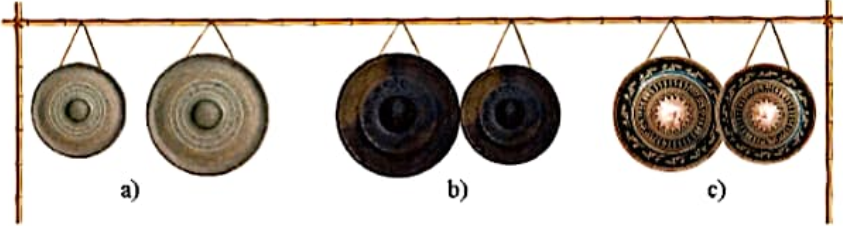
\includegraphics{images/Duongtron-H18}
	\end{center}
	\loigiai{
	\begin{itemize}
	\item Hình a) là hai đường tròn ngoài nhau. 
	\item Hình b) là hai đường tròn tiếp xúc ngoài. 
	\item Hình c) là hai đường tròn cắt nhau.
	\end{itemize}
	}
\end{vd}
%%==========Ví dụ 2
\begin{vd}
	Xác định vị trí tương đối của hai đường tròn $(O; R)$ và $(O'; R')$ trong mỗi trường hợp sau:
	\begin{listEX} [2]
	\item $OO'=12$; $R=5$; $R'=3$;
	\item $OO'=8$; $R=5$; $R'=3$;
	\item $OO'=7$; $R=5$; $R'=3$;
	\item $OO'=0$; $R=5$; $R'=4$.
	\end{listEX}
	\loigiai{
	\begin{listEX} [1]
	\item Ta có $12>5+3$ nên $OO'>R+R'$, suy ra hai đường tròn $(O ; R)$ và $(O'; R')$ ở ngoài nhau.
	\item Ta có $8=5+3$ nên $OO'=R+R'$, suy ra hai đường tròn $(O ; R)$ và $(O' ; R')$ tiếp xúc ngoài.
	\item Ta có $5-3<7<5+3$ nên $R-R'<O O'<R+R'$, suy ra hai đường tròn $(O ; R)$ và $(O' ; R')$ cắt nhau.
	\item Ta có $0<5$ nên $(OO'<R-R')$, suy ra đường tròn $(O ; R)$ đựng đường tròn $(O' ; R')$.
	\end{listEX}
	}
\end{vd}
%%==========Ví dụ 3
\begin{vd}
	Xác định vị trí tương đối giữa hai đường tròn $(I ; R)$ và $(J ; R')$ trong mỗi trường hợp sau:
	\begin{listEX}[2]
	\item $IJ=5$; $R=3$; $R'=2$;
	\item $IJ=4$; $R=11$; $R'=7$;
	\item $IJ=6$; $R=9$; $R'=4$;
	\item $IJ=10$; $R=4$; $R'=1$.
	\end{listEX}
	\loigiai{
	\begin{listEX} [1]
	\item Ta có $5=3+2$ nên $IJ'=R+R'$, suy ra hai đường tròn $(I ; R)$ và $(J; R')$ tiếp xúc ngoài. 
	\item Ta có $4=11-7$ nên $IJ=R-R'$, suy ra đường tròn $(I ; R)$ và $(J; R')$ tiếp xúc trong.
	\item Ta có $9-4<6<9+4$ nên $R-R'<IJ'<R+R'$, suy ra hai đường tròn $(I ; R)$ và $(J ; R')$ cắt nhau.
	\item Ta có $10>4+1$ nên $IJ'>R+R'$, suy ra hai đường tròn $(I ; R)$ và $(J; R')$ ở ngoài nhau.
	\end{listEX}
	}
\end{vd}
%%==========Ví dụ 4
\begin{vd}
	Cho hai điểm $O$ và $O'$ sao cho $OO'=5$ cm. Hãy giải thích tại sao hai đường tròn $\left(O;4 \,\text{cm} \right)$ và $\left(O';3 \,\text{cm} \right)$ cắt nhau.
	\loigiai{
	Đặt $R=4$ cm; $R'=3$ cm, ta thấy $1 \, \text{cm} \, < 5 \, \text{cm} \, < \, 7 \, \text{cm}$, nên 	$R-R'<OO'<R+R'$.\\
	Do đó, hai đường tròn đã cho cắt nhau.
	}
\end{vd}
%%==========Ví dụ 5
\begin{vd}
	Cho đường tròn $\left(O;5 \,\text{cm} \right)$ và điểm $I$ cách điểm $O$ một khoảng $2$ cm. Xác định vị trí tương đối của đường tròn đã cho và đường tròn $\left(I;r \right)$ trong mỗi trường hợp sau:
	\begin{listEX}[2]
	\item $r=4$ cm;
	\item $r=6$ cm.
	\end{listEX}
	\loigiai{
	\begin{enumerate}
	\item Đặt $R=5$ cm, ta thấy $1 \, \text{cm} \, < 2 \, \text{cm} \, < \,9 \, \text{cm}$, nên 	$R-r<OI<R+r$.\\
	Do đó, hai đường tròn đã cho cắt nhau.
	\item Đặt $R=5$ cm, ta thấy $1 \, \text{cm} \, < 2 \, \text{cm} \, < \,11 \, \text{cm}$, nên $r-R<OI<r+R$.\\
	Do đó, hai đường tròn đã cho cắt nhau.
	\end{enumerate}
	}
\end{vd}
%%==========Ví dụ 6
\begin{vd}
	Cho hai đường tròn $(O; 4\;\text{cm})$ và $(O'; 3\;\text{cm})$. Biết rằng $O O'=5$ cm. Xét vị trí tương đối của hai đường tròn đó.
	\loigiai{
	Ta thấy bán kính của hai đường tròn $(O)$; $(O')$ lần lượt là $R=4$ cm; $r=3$ cm.\\
	Do $R-r=4-3=1$; $R+r=4+3=7$ cm và $1<5<7$ nên $R-r<O O'<R+r$.\\
	Vậy hai đường tròn $(O ; 4\;\text{cm})$ và $(O'; 3\;\text{cm})$ cắt nhau.
	}
\end{vd}
%%==========Ví dụ 7
\begin{vd}
	Cho hai đường tròn $(O ; 14\;\text{cm})$; $(O'; 5\;\text{cm})$ với $O O'=8$ cm. Hỏi hai đường tròn đó có cắt nhau hay không?
	\loigiai{
	Ta thấy bán kính của hai đường tròn $(O)$; $(O')$ lần lượt là $R=14$ cm; $r=5$ cm.\\
	Do $R-r=14-5=9$; $R+r=14+5=19$ cm và $8 < 9 < 14$.\\
	Vậy hai đường tròn $(O ; 14\;\text{cm})$ và $(O'; 5\;\text{cm})$ không cắt nhau.	
	}
\end{vd}
%%==========Ví dụ 8
\begin{vd}
	Cho hai điểm $O$ và $O'$ sao cho $OO'=5$ cm. Giải thích tại sao hai đường tròn $\left(O;3\,\text{cm} \right)$ và $\left(O';2\,\text{cm} \right)$ tiếp xúc nhau. Chúng tiếp xúc trong hay tiếp xúc ngoài?
	\loigiai{
	Đặt $R=3$ cm, $R'=2$ cm ta thấy $5 \, \text{cm} = 2 \, \text{cm} +3 \, \text{cm}$, nghĩa là $OO'=R+R'$.\\
	Vậy hai đường tròn đã cho tiếp xúc ngoài với nhau.
	}
\end{vd}
%%==========Ví dụ 9
\begin{vd}
	Cho hai điểm $O$ và $O'$ sao cho $OO'=3$ cm. Giải thích tại sao hai đường tròn $\left(O;8\,\text{cm} \right)$ và $\left(O';5\,\text{cm} \right)$ tiếp xúc nhau. Chúng tiếp xúc trong hay tiếp xúc ngoài?
	\loigiai{
	Đặt $R=8$ cm, $R'=5$ cm ta thấy $3 \, \text{cm} = 8 \, \text{cm} -5 \, \text{cm}$, nghĩa là $OO'=R-R'$.\\
	Vậy hai đường tròn đã cho tiếp xúc trong với nhau.
	}
\end{vd}
%%==========Ví dụ 10
\begin{vd}
	Xác định vị trí tương đối của hai đường tròn $\left(O;3\,\text{cm} \right)$ và $\left(O';5\,\text{cm} \right)$ biết $OO'>8$ cm.
	\loigiai{
	Đặt $R=3$ cm, $R'=5$ cm ta có $OO'=8 \, \text{cm}>R+R'$.\\
	Vậy hai đường tròn đã cho là hai đường tròn ngoài nhau.
	}
\end{vd}
%%==========Ví dụ 11
\begin{vd}
	Cho hai điểm $O$ và $O'$ sao cho $OO'=2$ cm. Xác định vị trí tương đối của hai đường tròn $\left(O;5\,\text{cm} \right)$ và $\left(O';r \right)$ biết rằng $r<3$ cm.
	\loigiai{
	Đặt $R=3$ cm, vì $r<3$ nên $R-r=5-r>5-3=2=OO'$.\\
	Vậy đường tròn $\left(O;5\,\text{cm} \right)$ đựng đường tròn $\left(O';r \right)$.
	}
\end{vd}
%%==========Ví dụ 12
\begin{vd}%[9H2B7]
	Cho đường tròn tâm $O$, bán kính $R$. Lấy điểm $A$ tùy ý trên $(O)$. Vẽ đường tròn đường kính $OA$. Xác định vị trí tương đối của hai đường tròn.
	\loigiai
	{
	\immini{
	Gọi $O'$ là tâm đường tròn đường kính $OA$. Ta có $O'$ là trung điểm của $OA$ và bán kính đường tròn $(O')$ là $R'=\dfrac{OA}{2}=\dfrac{R}{2}$. Độ dài đoạn nối tâm $d=OO'=\dfrac{OA}{2}=\dfrac{R}{2}$. Ta có $R-R'=\dfrac{R}{2}=d$ nên $(O)$ và $(O')$ tiếp xúc trong tại $A$.}{
	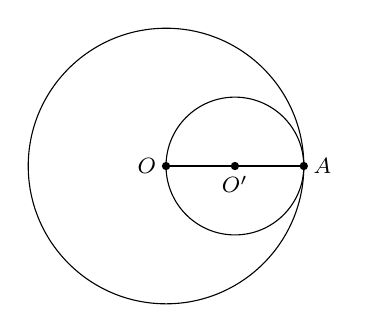
\begin{tikzpicture}[line join = round, line cap = round,>=stealth,font=\footnotesize,scale=1] 
	\def\R{1.75}
	\coordinate[label = left:$O$] (O) at (0,0); 
	\coordinate[label = right:$A$] (A) at (\R,0); 
	\coordinate[label = below:$O'$] (O') at (0.5*\R,0);
	\draw (O)--(A); 
	\draw (O) circle (\R);
	\draw (O') circle (0.5*\R);
	\foreach \x in {A,O,O'} \fill[black] (\x) circle (1.5pt); 
	\end{tikzpicture}
	}
	}
\end{vd}
%%==========Ví dụ 13
\begin{vd}%[9H2B7]
	Trong mặt phẳng tọa độ $Oxy$ cho hai điểm $A(-1;1)$ và $B(3;0)$. Vẽ các đường tròn $(A;r)$ và $(B;r')$. Khi $r=3$ và $r'=1$, hãy xác định vị trí tương đối của hai đường tròn.
	\loigiai
	{
	Độ dài đoạn nối tâm $d=AB=\sqrt{(3+1)^2+1^2}=\sqrt{17}$. \tagEX{1}
	Tổng hai bán kính $r+r'=3+1=4$. \tagEX{2}
	Từ $(1)$ và $(2)$ ta thấy $\sqrt{17}>4$ nên hai đường tròn không giao nhau; hai dường tròn $(A)$ và $(B)$ nằm ngoài nhau.
	}
\end{vd}
%%==========Ví dụ 14
\begin{vd}%[9H2K7]
	Cho $\triangle ABC$ có $\left(\widehat{B}, \widehat{C}\ne 90^\circ\right)$, đường cao $AH$. Từ $H$ kẻ $HK$ vuông góc với $AB$ tại $K$, $HI$ vuông góc với $AC$ tại $I$. Xác định vị trị tương đối của đường tròn ngoại tiếp $\triangle BHK$ và đường tròn ngoại tiếp $\triangle CHI$.
	\loigiai
	{
	\begin{center}
	\begin{tikzpicture}[line join = round, line cap = round,>=stealth,font=\footnotesize,scale=1.2]
	%, Hình 151
	\tkzDefPoints{0/0/B}
	\coordinate (C) at ($(B)+(6,0)$);
	\tkzDefShiftPoint[B](70:4){A}
	\tkzDefPointBy[projection = onto B--C](A) \tkzGetPoint{H}
	\tkzDefPointBy[projection = onto A--B](H) \tkzGetPoint{K}
	\tkzDefPointBy[projection = onto A--C](H) \tkzGetPoint{I}
	%
	\pgfresetboundingbox
	\tkzDrawSegments(A,B B,C C,A A,H H,K H,I)
	\tkzDrawPoints[fill=black](A,B,C,H,K,I)
	\tkzCircumCenter(K,B,H) \tkzGetPoint{O1} 
	\tkzCircumCenter(I,C,H) \tkzGetPoint{O2}
	\tkzDrawCircle[radius,black](O1,H) 
	\tkzDrawCircle[radius,black](O2,H) 
	\tkzDrawPoints[fill=black](O1,O2)
	\tkzDrawSegments[dashed](K,O1 I,O2)
	\tkzLabelPoints[above](A)
	\tkzLabelPoints[above left](K)
	\tkzLabelPoints[above right](I)
	\tkzLabelPoints[below](O1,O2)
	\tkzLabelPoints[below right](H)
	\tkzLabelPoints[left](B)
	\tkzLabelPoints[right](C)
	\tkzMarkSegments[mark=||](H,O2 C,O2)
	\tkzMarkSegments[mark=|](H,O1 B,O1)
	\tkzMarkRightAngles[size=0.2](A,K,H A,I,H)
	\path (K)--(O1) node[right,midway]{$R_1$};
	\path (I)--(O2) node[above left,midway]{$R_2$};
	\end{tikzpicture}
	\begin{tikzpicture}[line join = round, line cap = round,>=stealth,font=\footnotesize,scale=.9]
	%, Hình 152
	\tkzDefPoints{0/0/B}
	\coordinate (C) at ($(B)+(6,0)$);
	\tkzDefShiftPoint[B](120:4){A}
	\tkzDefPointBy[projection = onto B--C](A) \tkzGetPoint{H}
	\tkzDefPointBy[projection = onto A--B](H) \tkzGetPoint{K}
	\tkzDefPointBy[projection = onto A--C](H) \tkzGetPoint{I}	
	%
	\pgfresetboundingbox
	\tkzDrawSegments(A,B B,C C,A H,K H,I H,B)	
	\tkzDrawPoints[fill=black](A,B,C,H,K,I)
	\tkzCircumCenter(K,B,H) \tkzGetPoint{O1} 
	\tkzCircumCenter(I,C,H) \tkzGetPoint{O2} 
	\tkzDrawCircle[radius,black](O1,H) 
	\tkzDrawCircle[radius,black](O2,H) 
	\tkzDrawPoints[fill=black](O1,O2)
	\tkzDrawSegments[dashed](K,O1 I,O2 A,H)
	\tkzLabelPoints[above](A)
	\tkzLabelPoints[above right](K)
	\tkzLabelPoints[above](I)
	\tkzLabelPoints[below](O1,O2)
	\tkzLabelPoints[below right](B)
	\tkzLabelPoints[left](H)
	\tkzLabelPoints[right](C)
	\tkzMarkRightAngles[size=0.2](A,K,H A,I,H A,H,B)
	\path (K)--(O1) node[right,midway]{$R_1$};
	\path (I)--(O2) node[left,midway]{$R_2$};
	\end{tikzpicture}
	\end{center}
	\begin{itemize}
	\item \textit{Trường hợp 1.} \\
	Xét $\triangle ABC$ có $\widehat{B}<90^\circ$ và $\widehat{C}<90^\circ$. Gọi $O_1$, $O_2$ lần lượt là trung điểm của $BH$ và $CH$. Vì $\triangle BKH$ vuông tại $K$, $O_1$ là trung điểm của cạnh huyền $BH$ nên $KO_1=O_1B=O_1H=\dfrac{1}{2}BH=R_1$ $\Rightarrow \left(O_1;R_1\right)$ là đường tròn ngoại tiếp $\triangle BKH$. Tương tự, ta có $\left(O_2;R_2\right)$ là đường tròn ngoại tiếp $\triangle HIC$. Ta có, $R_1+R_2=O_1H+O_2H=O_1O_2$ nên $\left(O_1;R_1\right)$ tiếp xúc ngoài tại $H$ với $\left(O_2;R_2\right)$.
	\item \textit{Trường hợp 2.} Xét $\triangle ABC$ có $\widehat{B}=90^\circ$ (hoặc $\widehat{C}=90^\circ$). Lập luận tương tự như trường hợp 1 ta có $O_1O_2=R_2-R_1$ nên $\left(O_1;R_1\right)$ và $\left(O_2;R_2\right)$ tiếp xúc trong tại $H$.
	\end{itemize}	
	}
\end{vd}
%============
\begin{dang}{Chứng minh các tính chất về hệ thức hình học}
	%	\begin{itemize}
	%	\item Xác định vị trí của hai đường tròn.
	%	\item Dựa vào các tính chất đã biết để suy ra các tính chất và hệ thức hình học cần chứng minh.
	%	\end{itemize}
\end{dang}	
%%==========Ví dụ 15
\begin{vd}%[9H2K7]
	Cho hai đường tròn $(O;R)$ và $(O';R')$ tiếp xúc ngoài tại $A$. Kẻ tiếp tuyến chung ngoài $BC$, $B\in (O)$, $C\in (O')$. Tiếp tuyến chung trong tại $A$ cắt tiếp tuyến chung ngoài $BC$ tại $I$. Chứng minh rằng
	\begin{listEX}[2]
	\item $\widehat{OIO'}=90^\circ$;
	\item $BC=2\sqrt{RR'}$.
	\end{listEX}
	\loigiai
	{\immini{
	\vspace*{-0.5cm}
	\begin{enumerate}
	\item Ta có $IB$, $IA$ là hai tiếp tuyến của $(O)$ nên $\widehat{I_1}=\widehat{I_2}$; $IC$, $IA$ là hai tiếp tuyến của $(O')$ nên $\widehat{I_3}=\widehat{I_4}$. \\Suy ra $\widehat{OIO'}=\widehat{I_2}+\widehat{I_3}=180^\circ:2=90^\circ$.
	\item Ta có $IB$, $IA$ là hai tiếp tuyến của $(O)$ nên $IB=IA$ và $IA\perp OA$, $IC$, $IA$ là hai tiếp tuyến của $(O')$ nên $IC=IA$ và $IA\perp O'A$. Suy ra $IA=IB=IC$. Ba điểm $O$, $A$, $O'$ thẳng hàng và $IA\perp OO'$. Áp dụng hệ thức $h^2=b'\cdot c'$ vào tam giác vuông $OIO'$ , ta có $IA^2=OA\cdot O'A\Rightarrow IA=\sqrt{R\cdot R'}$. Mặt khác $BC=IB+IC=2IA$ nên $BC=2\sqrt{R\cdot R'}$.
	\end{enumerate}}{\begin{tikzpicture}[line join = round, line cap = round,>=stealth,font=\footnotesize,scale=0.7]
	\tkzDefPoints{0/0/O}
	\coordinate (O') at ($(O)+(6,0)$);
	\tkzDefTriangle[two angles = 55 and 35](O,O') \tkzGetPoint{I}
	\tkzDefPointBy[projection = onto O--O'](I)
	\tkzGetPoint{A}
	\tkzDefCircle[diameter](O,I) \tkzGetPoint{M} 
	\tkzDefCircle[diameter](O',I) \tkzGetPoint{N} 
	\tkzInterCC(M,O)(O,A) \tkzGetSecondPoint{B}
	\tkzInterCC(N,O')(O',A) \tkzGetFirstPoint{C}
	%
	\pgfresetboundingbox
	\tkzDrawSegments(B,C I,A)
	\tkzDrawPolygon(I,O,O')
	\tkzDrawPoints[fill=black](I,O,O',A,B,C)
	\tkzDrawCircle[radius](O,A)
	\tkzDrawCircle[radius](O',A)
	\tkzLabelPoints[above](I,B,C)
	\tkzLabelPoints[left](O)
	\tkzLabelPoints[right](O')
	\tkzLabelPoints[above right](A)
	\tkzLabelAngles[pos=0.7,rotate=30](B,I,O){\scriptsize $1$}
	\tkzLabelAngles[pos=0.7,rotate=30](O,I,A){\scriptsize $2$}
	\tkzLabelAngles[pos=0.7,rotate=30](A,I,O'){\scriptsize $3$}
	\tkzLabelAngles[pos=0.7,rotate=30](O',I,C){\scriptsize $4$}
	\end{tikzpicture}}
	}
\end{vd}
%%==========Ví dụ 16
\begin{vd}%[9H2G7]
	Cho hai đường tròn $(O)$ và $(O')$ cắt nhau tại $A$ và $B$, trong đó $O'$ nằm trên đường tròn $(O)$. Kẻ đường kính $O'C$ của đường tròn $(O)$.
	\begin{enumerate}
	\item Chứng minh rằng $CA$, $CB$ là hai tiếp tuyến của $(O')$.
	\item Đường vuông góc với $AO'$ tại $O'$ cắt $CB$ tại $I$. Đường vuông góc với $AC$ tại $C$ cắt đường thẳng $O'B$ ở $K$. Chứng minh rằng ba điểm $O$, $I$, $K$ thẳng hàng.
	\end{enumerate}
	\loigiai
	{
	\immini{\vspace*{-1cm}
	\begin{enumerate}
	\item Tam giác $CAO'$ có đường trung tuyến $AO$ ứng với cạnh $CO'$ bằng nửa cạnh $CO'$ nên $\widehat{CAO'}=90^\circ$. Mà $A\in (O')$ nên $CA$ là tiếp tuyến của $(O')$ tại $A$.\\
	Tương tự ta có $CB$ là tiếp tuyến của $(O')$.
	\item Theo tính chất hai tiếp tuyến cắt nhau thì $\widehat{C_1}=\widehat{C_2}$. \tagEX{1}
	Ta có $CA\parallel IO'$ (cùng vuông góc với $O'A$) nên $\widehat{C_1}=\widehat{O_1'}$. \tagEX{2}
	Từ $(1)$ và $(2)$ suy ra $\widehat{C_2}=\widehat{O_1'}$. Do đó, $IC=IO'$. \tagEX{3}
	Theo tính chất hai tiếp tuyến cắt nhau thì $\widehat{O_2'}=\widehat{CO'B}$. Mặt khác $CK\parallel AO'$ (cùng vuông góc với $AC$) nên $\widehat{O_2'}=\widehat{O;CK}$. Suy ra $\widehat{CO'B}=\widehat{O'CK}$. Do đó, $KC=KO'$. \tagEX{4}
	Mà $OC=OO'$ (vì $O'$, $C$ cùng thuộc $(O)$). \tagEX{5}
	Từ $(3)$, $(4)$, $(5)$ suy ra $O$, $I$, $K$ cùng thuộc đường trung trực của $CO'$.\\ Vậy ba điểm $I$, $O$, $K$ thẳng hàng.
	\end{enumerate}}{\begin{tikzpicture}[line join = round, line cap = round,>=stealth,scale=.8]
	%, Hình 154
	\tkzDefPoints{0/0/O}
	\tkzDefShiftPoint[O](0:2){O'}
	\tkzDefShiftPoint[O](0:0.4){M}
	\tkzDefPointBy[symmetry = center O](O') \tkzGetPoint{C}
	\tkzInterCC(O,C)(O',M) \tkzGetPoints{A}{B}
	\tkzDefPointWith[orthogonal,K=3](O',A) \tkzGetPoint{N}
	\tkzInterLL(C,B)(O',N) \tkzGetPoint{I}
	\tkzDefPointWith[orthogonal,K=3](C,A) \tkzGetPoint{P}
	\tkzInterLL(C,P)(O',B) \tkzGetPoint{K}
	\pgfresetboundingbox
	\tkzDrawCircle[radius](O,C)
	\tkzDrawCircle[radius](O',M)
	\tkzDrawSegments(C,O' C,A C,B O',A O',B O',I C,K B,K)
	\tkzDrawSegments[dashed](O,K)
	\tkzDrawPoints[fill=black](C,O',O,A,B,I)
	\tkzLabelPoints[left](C)
	\tkzLabelPoints[right](O',K)
	\tkzLabelPoints[above](O)
	\tkzLabelPoints[above right](A)
	\tkzLabelPoints[below right](B)
	\tkzLabelPoints[below left](I)
	\tkzMarkRightAngles[size=0.2](A,O',I C,A,O' A,C,K)
	\tkzLabelAngles[pos=-0.8,rotate=0](A,C,O){\scriptsize $1$}
	\tkzLabelAngles[pos=-0.8,rotate=0](O,C,B){\scriptsize $2$}
	\tkzLabelAngles[pos=0.8,rotate=0](O,O',I){\scriptsize $1$}
	\tkzLabelAngles[pos=0.8,rotate=0](A,O',C){\scriptsize $2$}
	\end{tikzpicture}}
	}
\end{vd}
%%==========Ví dụ 17
\begin{vd}%[9H2G7]
	Cho hai đường tròn $\left(O_1;R_1\right)$ và $\left(O_2;R_2\right)$ (với $R_1\ne R_2$) tiếp xúc ngoài tại $A$. Kẻ các tiếp tuyến chung ngoài $BC$ và $DE$ (với $B$, $D$ thuộc $(O_1)$; $C$, $E$ thuộc $(O_2)$). Chứng minh rằng $BC+DE=BD+CE$.	
	\loigiai{
	\begin{center}
	\begin{tikzpicture}[line join = round, line cap = round,>=stealth,scale=1]
	%, Hình 155
	\tkzDefPoints{0/0/O1}
	\tkzDefPoints{2.5/0/A}
	\tkzDefPoints{4/0/O2}
	\tkzDefPointWith[orthogonal,K=1.5](A,O1) \tkzGetPoint{P}
	\pgfresetboundingbox
	\tkzDrawPoints[fill=black](O1,O2,A)
	\tkzDrawCircle[radius,black](O1,A)
	\tkzDrawCircle[radius,black](O2,A)
	\tkzInterLC[R](O1,O2)(O1,1 cm) \tkzGetSecondPoint{g}
	\tkzDefTangent[from=O2](O1,g) \tkzGetPoints{b}{a}
	\tkzInterLC[R](O1,a)(O1,2.5 cm) \tkzGetSecondPoint{B}
	\coordinate (C) at ($(B)+(O2)-(a)$);
	\tkzInterLC[R](O1,b)(O1,2.5 cm) \tkzGetSecondPoint{D}
	\coordinate (E) at ($(D)+(O2)-(b)$);
	\tkzInterLL(A,P)(C,B) \tkzGetPoint{M}
	\tkzDefPointBy[symmetry = center A](M) \tkzGetPoint{N}
	%\tkzDrawSegments()
	\tkzDrawSegments[dashed](O1,O2 O1,B O1,D O2,C O2,E)
	\tkzDrawSegments(B,C D,E B,D C,E M,N)
	\tkzDrawPoints[fill=black](O1,O2,A,B,C,D,E,M,N)
	\tkzMarkSegments[mark=|](B,M M,C D,N N,E)
	\tkzMarkRightAngles[size=0.2](M,B,O1 M,C,O2 N,D,O1 N,E,O2)
	\tkzLabelPoints[below](D,E,N)
	\tkzLabelPoints[above](B,M,C)
	\tkzLabelPoints[left](O1)
	\tkzLabelPoints[below left](A,O2)
	\end{tikzpicture}
	\end{center}
	Vẽ tiếp tuyến chung tại $A$ lần lượt cắt $BC$, $DE$ tại $M$ và $N$. Vì $MA$, $MB$ là tiếp tuyến của $(O_1)$ nên $MA=MB$. Vì $MA$, $MC$ là tiếp tuyến của $(O_2)$ nên $MA=MC\Rightarrow MA=MB=MC$.\\Chứng minh tương tự ta có $NA=ND=NE$. $\Rightarrow BC+DE=2MN$. \tagEX{1}
	Gọi giao điểm của $BC$ và $DE$ là $K$, khi đó $K$ thuộc đường thẳng $O_1O_2$ $\Rightarrow KB=KD$ (tính chất hai tiếp tuyến cắt nhau).	Mà $O_1B=O_1D=R_1$ nên $KO_1$ là trung trực của đoạn $BD$ suy ra $O_1O_2\perp BD$.\\ Chứng minh tương tự ta được $O_1O_2\perp CE$.Suy ra tứ giác $BCED$ là hình thang (vì $BD\parallel CE$). Vì $M$, $N$ lần lượt là trung điểm của $BC$ và và $DE$ nên $2MN=BD+CE$. \tagEX{2}
	Từ $(1)$ và $(2)$ suy ra $BC+DE=BD+CE$.
	}
\end{vd}
%%==========Ví dụ 18
\begin{vd}%[9H2G7]
	Cho hai đường tròn $(O_1)
	$, $(O_2)$ ngoài nhau. Vẽ các tiếp tuyến chung ngoài $AB$ và $CD$ (với $A$, $D$ thuộc $(O_1)$; $B$, $C$ thuộc $(O_2)$). Nối $AC$ cắt $(O_1)$ tại $M$; cắt $(O_2)$ tại $N$ ($M\ne A, N\ne C$). Chứng minh rằng $AM=NC$.	
	\loigiai{
	Vẽ đường trung trực $d$ của đoạn $AB$, $d$ cắt $O_1O_2$ tại $I$. Khi đó $IA=IB$. Ta có $B$ và $C$ đối xứng nhau qua $O_1O_2$ nên $IB=IC$ $\Rightarrow IA=IC$. 
	\immini{
	Kẻ $IH\perp AC$ tại $H$ ta có $HA=HC$ (vì $\triangle IAC$ cân tại $I$). Kẻ $O_1K\perp AC$ tại $K$, $O_2G\perp AC$ tại $G$ $\Rightarrow O_1K\parallel IH\parallel O_2G$. Xét hình thang $ABO_2O_1$ (vì $O_1A\parallel O_2G$ do cùng vuông góc với $AB$) ta có $d\parallel AO_1\parallel BO_2$ và $d$ đi qua trung điểm của $AB$ nên $d$ đi qua trung điểm của $O_1O_2$ hay $I$ là trung điểm của $O_1O_2$.\\ Xét hình thang $O_1KO_2G$ có $IH\parallel O_1K\parallel O_2G$ và $I$ là trung điểm của $O_1O_2$ nên $H$ là trung điểm của $KG$ $\Rightarrow HK=HG\Rightarrow HA-HK=HC-HG$ hay $AK=GC$ $\Rightarrow 2AK=2GC\Rightarrow AM=CN$.
	\begin{note}{Trong ví dụ này ta đã sử dụng tính chất đường thẳng song song với hai đáy của hình thang và đi qua trung điểm của một đường chéo thì đi qua trung điểm của đường chéo còn lại}
	\end{note} 
	}{\begin{tikzpicture}[line join = round, line cap = round,>=stealth,scale=0.85]
	%, Hình 156
	\tkzDefPoints{0/0/O1}
	\tkzDefPoints{2.5/0/X}
	\tkzDefPoints{6/0/O2}
	\tkzDefPoints{4.5/0/Y}
	\pgfresetboundingbox
	\tkzDrawPoints[fill=black](O1,O2,A)
	\tkzDrawCircle[radius,black](O1,X)
	\tkzDrawCircle[radius,black](O2,Y)
	\tkzInterLC[R](O1,O2)(O1,1 cm) \tkzGetSecondPoint{g}
	\tkzDefTangent[from=O2](O1,g) \tkzGetPoints{b}{a}
	\tkzInterLC[R](O1,a)(O1,2.5 cm) \tkzGetSecondPoint{A}
	\coordinate (B) at ($(A)+(O2)-(a)$);
	\tkzInterLC[R](O1,b)(O1,2.5 cm) \tkzGetSecondPoint{D}
	\coordinate (C) at ($(D)+(O2)-(b)$);
	\tkzInterLC(A,C)(O1,X) \tkzGetPoints{M}{}
	\tkzInterLC(C,A)(O2,Y) \tkzGetPoints{N}{}
	\coordinate (Z) at ($(A)!0.5!(B)$);
	\tkzDefPointWith[orthogonal,K=1.5](Z,A) \tkzGetPoint{P}
	\tkzInterLL(Z,P)(O1,O2) \tkzGetPoint{I}
	\tkzDefPointBy[projection = onto A--C](I) \tkzGetPoint{H}
	\tkzDefPointBy[projection = onto A--C](O1) \tkzGetPoint{K}
	\tkzDefPointBy[projection = onto A--C](O2) \tkzGetPoint{G}
	%\tkzDrawSegments()
	%\tkzDrawSegments[dashed](O1,O2 O1,B O1,D O2,C O2,E)
	\tkzDrawSegments(A,B D,C O1,O2 A,C O1,A O2,B O1,K O2,G I,H Z,I)
	\tkzDrawPoints[fill=black](O1,O2,A,B,C,D,M,N,Z,I,H,K,G)
	\tkzMarkRightAngles[size=0.2](A,K,O1 C,G,O2 I,H,M B,Z,I)
	\tkzLabelPoints[below](D,C,K,I)
	\tkzLabelPoints[above](B,A,H)
	\tkzLabelPoints[above right](M)
	\tkzLabelPoints[left](O1)
	\tkzLabelPoints[below left](N)
	\tkzLabelPoints[below right](O2)
	\tkzLabelPoints[below](G)
	\tkzMarkSegments[mark=||](Z,A Z,B)
	\end{tikzpicture}}
	}
\end{vd}
\begin{dang}{Tính độ dài đoạn thẳng}
	%\begin{itemize}
	%\item Vận dụng tính chất tiếp tuyến, tiếp tuyến chung, hai tiếp tuyến cắt nhau và tính chất đoạn nối tâm.
	%\item Áp dụng định lí Pi-ta-go, hệ thức lượng trong tam giác vuông và tỉ số lượng giác của góc nhọn.
	%\end{itemize}
\end{dang}
%%==========Ví dụ 19
\begin{vd}%[9H2B8]
	\immini{
	Trong hình vẽ, cho hai đường tròn đồng tâm $O$. Cho biết $BC$ là đường kính của đường tròn lớn và có độ dài bằng $8$. Dây $CD$ là tiếp tuyến của đường tròn nhỏ và $\widehat{BCD}=30^\circ$. Hãy tính bán kính của đường tròn nhỏ.}
	{\begin{tikzpicture}[line join = round, line cap = round,>=stealth,scale=1]
	\tkzDefPoints{0/0/O}
	\tkzDefShiftPoint[O](0:2){C}
	\tkzDefPointBy[symmetry = center O](C) \tkzGetPoint{B}
	\tkzDefTriangle[two angles = 30 and 60](C,B) \tkzGetPoint{D}
	\tkzDefPointBy[projection = onto D--C](O) \tkzGetPoint{M}
	\pgfresetboundingbox
	\tkzDrawCircle[radius,black](O,C)
	\tkzDrawCircle[radius,black](O,M)
	\tkzDrawSegments(C,B C,D O,M)
	\tkzDrawPoints[fill=black](C,B,O,D,M)
	\tkzLabelPoints[left](B)
	\tkzLabelPoints[right](C)
	\tkzLabelPoints[below](O,D)
	\tkzLabelPoints[below right](M)
	\tkzLabelAngles[pos=0.6](B,C,D){\tiny$30^\circ$}
	\tkzMarkRightAngles[size=0.2](O,M,C)
	\end{tikzpicture}}
	\loigiai
	{
	Ta có $BC=8$ nên bán kính đường tròn lớn là $OC=4$. Vì $CD$ là tiếp tuyến của đường tròn nhỏ, nên $CD \perp OM.$\\
	Do đó $OM=OC \cdot \sin 30^\circ = 4 \cdot \dfrac{1}{2}=2.$
	}
\end{vd}
%%==========Ví dụ 20
\begin{vd}%[9H2B8]
	Cho hai đường tròn $(O; R)$ và $(O'; R)$ cắt nhau tại $M$ và $N$. Biết $OO'=24$ cm, $MN=10$ cm. Tính $R$.
	\loigiai
	{
	\immini{Gọi giao điểm của $OO'$ và $MN$ là $I$. Vì $OM=ON=O'M=O'N=R$ nên tứ giác $OMO'N$ là hình thoi $\Rightarrow\; OO' \perp MN$ tại điểm $I$ là trung điểm của mỗi đoạn $OO'$ và $MN$.\\
	Do đó $IM=\frac{1}{2} MN = 5 \text{ cm},\; IO=\frac{1}{2}OO'=12\text{ cm.}$\\
	Áp dụng định lí Py-ta-go vào $\triangle MIO$, ta có: $$R=OM=\sqrt{IM^2+IO^2}=\sqrt{5^2+12^2}=13 \text{ (cm)}.$$
	Vậy $R=13$ cm.
	}
	{\begin{tikzpicture}[line join = round, line cap = round,>=stealth,scale=1]
	\tkzDefPoints{0/0/O}
	\tkzDefShiftPoint[O](0:2){A}
	\tkzDefShiftPoint[O](0:3){O'}
	\tkzDefShiftPoint[O'](0:-2){B}
	\tkzInterCC(O,A)(O',B) \tkzGetPoints{M}{N}
	\tkzInterLL(M,N)(O,O') \tkzGetPoint{I}
	\pgfresetboundingbox
	\tkzDrawCircle[radius,black](O,A)
	\tkzDrawCircle[radius,black](O',B)
	\tkzDrawSegments(O,O' M,N)
	\tkzDrawSegments[dashed](O,M O,N O',M O',N)
	\tkzDrawPoints[fill=black](O,O',M,N,I)
	\tkzLabelPoints[left](O)
	\tkzLabelPoints[right](O')
	\tkzLabelPoints[above](M)
	\tkzLabelPoints[below](N)
	\tkzLabelPoints[below left](I)
	\tkzMarkRightAngles[size=0.2](M,I,O')
	\end{tikzpicture}}
	}
\end{vd}
%%==========Ví dụ 21
\begin{vd}%[9H2B8]
	Cho hai đường tròn $(O; R)$ và $(O'; R')$ tiếp xúc ngoài tại $A$. Kẻ tiếp tuyến chung ngoài $MN$ với $M$ thuộc $(O)$, $N$ thuộc $(O')$. Biết $R=9$ cm, $R'=4$ cm. Tính độ dài đoạn $MN$.
	\loigiai
	{
	\immini{
	Ta có: $OO'=OA+O'A=9+4=13$ (cm).\\
	Kẻ $OH \perp OM$ tại $H$\\
	$\Rightarrow$ tứ giác $O'NMH$ là hình chữ nhật\\
	$\Rightarrow\; MH=O'N=4$ (cm); $MN=O'H$\\
	$\Rightarrow\; OH=OM-MH=9-4=5$ (cm).\\
	Áp dụng định lí Py-ta-go vào $\triangle OO'H$, ta có: $$MN=O'H=\sqrt{OO'^2-OH^2}=\sqrt{13^2-5^2}=12 \text{ (cm)}.$$
	%Vậy $MN=12$ cm.
	}
	{\vspace*{3mm}
	\begin{tikzpicture}[line join = round, line cap = round,>=stealth,scale=0.5]
	\tkzDefPoints{0/0/O}
	\tkzDefPoints{4.5/0/A}
	\tkzDefPoints{6.5/0/O'}
	\pgfresetboundingbox
	\tkzDrawPoints[fill=black](O,O',A)
	\tkzDrawCircle[radius,black](O,A)
	\tkzDrawCircle[radius,black](O',A)
	\tkzInterLC[R](O,O')(O,2.5 cm) \tkzGetSecondPoint{g}
	\tkzDefTangent[from=O'](O,g) \tkzGetPoints{b}{a}
	\tkzInterLC[R](O,a)(O,4.5 cm) \tkzGetSecondPoint{M}
	\coordinate (N) at ($(M)+(O')-(a)$);
	\tkzDefPointBy[projection = onto O--M](O') \tkzGetPoint{H}
	\tkzDefEquilateral(O,M) \tkzGetPoint{C}
	\tkzDrawArc[dashed](C,O)(M)
	\tkzInterLC(O',H)(C,O) \tkzGetSecondPoint{9}
	\tkzDrawSegments(O,O' O,M O',N M,N O',H)
	\tkzDrawPoints[fill=black](O,O',M,N,H)
	\tkzMarkRightAngles[size=0.2](O',N,M O,M,N M,H,O')
	\tkzLabelPoints[above](M,N)
	\tkzLabelPoints[left](O,H)
	\tkzLabelPoints[below left](A,O')
	\path (O)--(A) node[above,midway,sloped]{$9$};
	\path (A)--(O') node[above,midway,sloped]{$4$};
	\end{tikzpicture}}
	}
\end{vd}
%%==========Ví dụ 22
\begin{vd}%[9H2B8]
	Cho hai đường tròn ($O$; $3$ cm) và ($O'$; $4$ cm) cắt nhau tại $A$ và $B$. Qua $A$ kẻ một cát tuyến cắt $(O)$ tại $M$ ($M \ne A$), cắt ($O'$) tại $N$ ($N \ne A$). Nếu $OO' = 5$ cm, hãy tính giá trị lớn nhất của $MN$.
	\loigiai
	{
	\immini{
	Kẻ $OH \perp AM$ tại $H$, $O'K \perp AN$ tại $K$ và $OI\perp O'K$ tại $I$\\
	$\Rightarrow\; HM=HA$, $KA=KN$ và tứ giác $HOIK$ là hình chữ nhật\\
	$\Rightarrow\; MN=2HK$ và $HK=OI.$\\
	Ta có $OI \leq OO'$ (đường vuông góc và đường xiên\\
	$\Rightarrow MN=2HK=2OI \leq 2OO'=10$ (cm)\\
	Dấu $''=''$ xảy ra $\Leftrightarrow\; OI=OO' \Leftrightarrow I \equiv O' \Leftrightarrow d \parallel OO'.$\\
	Vậy giá trị lớn nhất của $MN$ bằng $10$ cm khi cát tuyến $d$ song song với $OO'.$}
	{\vspace*{-3mm}
	\begin{tikzpicture}[line join = round, line cap = round,>=stealth,scale=0.6]
	\tkzDefPoints{0/0/O}
	\tkzDefShiftPoint[O](0:3){P}
	\tkzDefShiftPoint[O](0:5){O'}
	\tkzDefShiftPoint[O'](0:-4){Q}
	\tkzInterCC(O,P)(O',Q) \tkzGetPoints{A}{B}
	\tkzDefPointBy[rotation = center O angle 105](A) \tkzGetPoint{M}
	\tkzInterLC(M,A)(O',A) \tkzGetPoints{N}{}
	\tkzDefPointBy[projection = onto A--M](O) \tkzGetPoint{H}
	\tkzDefPointBy[projection = onto A--N](O') \tkzGetPoint{K}
	\tkzDefPointBy[projection = onto K--O'](O) \tkzGetPoint{I}
	\coordinate (d) at ($(K)!1.3!(N)$);
	\pgfresetboundingbox
	\tkzDrawCircle[radius,black](O,P)
	\tkzDrawCircle[radius,black](O',Q)
	\tkzDrawSegments(O,O' M,N O,H O',K O,I N,d)
	%\tkzDrawSegments[dashed](O,M O,N O',M O',N)
	\tkzDrawPoints[fill=black](O,O',A,B,M,N,H,K,I)
	\tkzLabelPoints[left](O,M)
	\tkzLabelPoints[right](O',I)
	\tkzLabelPoints[above](A,H,K,d,N)
	\tkzLabelPoints[below](B)
	\tkzMarkRightAngles[size=0.2](M,H,O N,K,O' O,I,O')
	\tkzMarkSegments[mark=||](K,A K,N)
	\tkzMarkSegments[mark=|](M,H H,A)
	\end{tikzpicture}}
	}
\end{vd}
%%%%%%%%%%%%%%%%%%%
\subsection{Bài tập vận dụng}
%%==========Bài 2
\begin{bt}
	Trong mặt phẳng tọa độ $Oxy$, cho các điểm $M(0;2)$, $N(0;-3)$ và $P(2;-1)$. Vẽ hình và cho biết trong các điểm đã cho, điểm nào nằm trên, điểm nào nằm trong, điểm nào nằm ngoài đường tròn $\left(O;\sqrt5\right)$? Vì sao?
	\loigiai{
	\immini{
	Dựa vào hình vẽ ta thấy
	\begin{itemize}
	\item Điểm $M$ nằm trong đường tròn $\left(O;\sqrt5\right)$.
	\item Điểm $N$ nằm ngoài đường tròn $\left(O;\sqrt5\right)$.
	\item Điểm $P$ nằm trên đường tròn $\left(O;\sqrt5\right)$.
	\end{itemize}
	}{
	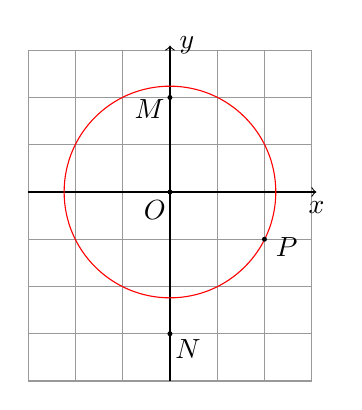
\begin{tikzpicture}[scale=0.6]
	\draw[step=1cm,color=black!40] (-3,-4) grid (3,3);
	\draw[->] (-3,0)--(3.1,0) node[below] {$x$};
	\draw[->] (0,-4)--(0,3.1) node[right] {$y$};
	\coordinate (O) at (0,0);
	\coordinate (M) at (0,2);
	\coordinate (N) at (0,-3);
	\coordinate (P) at (2,-1);
	\draw[red] (O) circle [radius=2.24];
	\foreach \p/\g in {M/-150,N/-40,P/-20,O/-130} 
	\fill (\p) circle(1.5pt) node [shift={(\g:.3)}] {$\p$}; 
	\end{tikzpicture}
	}
	}
\end{bt}
%%==========Bài 1
\begin{bt}
	Cho đường tròn $(O)$, bán kính $5$ cm và bốn điểm $A$, $B$, $C$, $D$ thỏa mãn $OA=3$ cm, $OB=4$ cm, $OC=7$ cm, $OD=5$ cm. Hãy cho biết mỗi điểm $A$, $B$, $C$, $D$ nằm trong, nằm trên hay nằm ngoài đường tròn $(O)$.
	\loigiai{
	\immini{\begin{itemize}
	\item $OA=3<R=5$ nên điểm $A$ ở trong đường tròn.
	\item $OB=4<R=5$ nên điểm $B$ ở trong đường tròn.
	\item $OC=7>R=5$ nên điểm $C$ ở ngoài đường tròn.
	\item $OD=5=R=5$ nên điểm $D$ ở trên đường tròn.
	\end{itemize}}{\begin{tikzpicture}[scale=0.4]
	\def\r{5}
	\def\u{4}
	\def\v{7}
	\def\t{3}
	\path
	(0:0) coordinate (O)
	(60:\u) coordinate (B)
	(100:\v) coordinate (C)
	(150:\t) coordinate (A)
	(30:\r) coordinate (D)
	;
	\draw[black] (O) circle (\r);
	\foreach \x/\g in {D/45,O/0,A/90,B/90,C/90}
	\draw [fill= white] (\x) circle (.05)+(\g:.5) node{$\x$};
	\end{tikzpicture}}
	}
\end{bt}
%%==========Bài 3
\begin{bt}
	Cho hai đường tròn $(A ; 6 \mathrm{~cm})$ và $(B ; 4 \mathrm{~cm})$ cắt nhau tại $C$ và $D$, $AB=8 \mathrm{~cm}$. Gọi $K$, $I$ lần lượt là giao điểm của hai đường tròn đâ cho với đoạn thẳng $AB$.
	\begin{listEX} [1]
	\item Tính độ dài của các đoạn thẳng $CA$, $CB$, $DA$ và $DB$.
	\item Điểm $I$ có phải là trung điểm của đoạn thẳng $AB$ không?
	\item Tính độ dài của đoạn thẳng $IK$.
	\end{listEX}
	\loigiai{
	\immini{\begin{listEX} [1]
	\item Hai đường tròn $(A ; 6 \mathrm{~cm})$ và $(B ; 4 \mathrm{~cm})$ cắt nhau tại $C$ và $D$ nên $AC=AD=6$ cm, $BC=BD=4$ cm.
	\item $AB=8$ cm. $BC=BD=BI=4$ cm. Suy ra $AI=AB-IB= 8-4=4$ cm. Điểm $I$ là trung điểm của đoạn thẳng $AB$.
	\item Ta có $AK=AC=6$ cm nên $IK=AK-AI=6-4=2$ cm.
	\end{listEX}}{	\begin{tikzpicture}[scale=0.32]
	\def\r{6}
	\def\v{4}
	\path
	(0:0) coordinate (A)
	(0:8) coordinate (B)
	(0:4) coordinate (I)
	(0:6) coordinate (K)
	;
	\draw[black] (A) circle (\r);
	\draw[black] (B) circle (\v);
	\path[name path=c1] (A) circle (\r);
	\path[name path=c2] (B) circle (\v);
	\path[name intersections={of=c1 and c2,by={C,D}}]; 
	\draw (A)--(C)--(B)--(A)--(D)--(B);
	\foreach \x/\g in {D/-90,B/0,A/180,C/80,I/135,K/45}
	\draw [fill= white] (\x) circle (.05)+(\g:.5) node{$\x$};
	\end{tikzpicture}}
	}
\end{bt}
%%==========Bài 4
\begin{bt}
	Cho hai đường tròn $(O ; 2 \mathrm{cm})$ và $(A ; 2 \mathrm{cm})$ cắt nhau tại $C$, $D$, điểm $A$ nằm trên đường tròn tâm $O$.
	\begin{listEX} [1]
	\item Vẽ đường tròn $(C ; 2 \mathrm{~cm})$.
	\item Đường tròn $(C ; 2 \mathrm{~cm})$ có đi qua hai điểm $O$ và $A$ không? Vì sao?
	\end{listEX}
	\loigiai{
	\immini{
	\begin{listEX} [1]
	\item Vẽ đường tròn $(C ; 2 \mathrm{~cm})$ (Hình bên).
	\item Đường tròn $(O ; 2 )$ và $(A ; 2 )$ cắt nhau tại $C$, $D$, điểm $A$ nằm trên đường tròn tâm $O$ nên $OC=OD=2$ cm, $AC=AD=2$ cm.\\
	Suy ra $CO=CA=2$ cm. Do đó đường tròn $(C ; 2 \mathrm{~cm})$ đi qua hai điểm $O$ và $A$.
	\end{listEX}}{\begin{tikzpicture}[scale=0.7]
	\def\r{2}
	\def\v{2}
	\def\u{2}
	\path
	(0:0) coordinate (O)
	(0:\r) coordinate (A)
	;
	\draw[black] (O) circle (\r);
	\draw[black] (A) circle (\v);
	\path[name path=c1] (O) circle (\r);
	\path[name path=c2] (A) circle (\v);
	\path[name intersections={of=c1 and c2,by={C,D}}]; 
	\draw[black] (C) circle (\u);
	\foreach \x/\g in {D/-90,O/180,A/0,C/90}
	\draw [fill= white] (\x) circle (.05)+(\g:.5) node{$\x$};
	\end{tikzpicture}}
	}
\end{bt}
%%==========Bài 5
\begin{bt}%[9H2K1]
	Cho tam giác $ABC$, cạnh $BC$ cố định, $AB=4$ cm.
	\begin{enumerate}
	\item Hỏi điểm $A$ di động trên đường nào ?
	\item Trung điểm $M$ của $AC$ di động trên đường nào ?
	\end{enumerate}
	\loigiai{
	\immini{
	\begin{enumerate}
	\item Điểm $B$ cố định. Điểm $A$ cách $B$ một khoảng là $4$ cm nên $A$ nằm trên đường tròn $(B;4\text{ cm})$.
	\item Gọi $O$ là trung điểm của $BC$ thì $O$ là một điểm cố định. Ta có $OM=\dfrac{1}{2}AB=2$ cm. Điểm $M$ cách điểm $O$ một khoảng $2$ cm nên $M$ nằm trên đường tròn $(O;2\text{ cm})$.
	\end{enumerate}
	}{
	\begin{tikzpicture}[scale=0.6, font=\footnotesize, line join=round, line cap=round, >=stealth]
	\tikzset{label style/.style={font=\footnotesize}}
	\tkzDefPoints{0/0/B,3/0/O}
	\tkzDrawCircle(B,O)
	\tkzDefPointBy[rotation = center B angle 60](O) \tkzGetPoint{A}
	\tkzDefTangent[at=A](B) \tkzGetPoint{t}
	\tkzDefPointBy[projection = onto A--t](O) \tkzGetPoint{M}
	\tkzDrawCircle[dashed](O,M)
	\tkzInterLL(A,M)(B,O) \tkzGetPoint{C}
	\tkzDrawPoints[fill=black](A,B,O,M,C)
	\tkzDrawSegments[](A,C O,M A,B B,C)
	\tkzMarkSegments[mark=|,size=0.1](B,O C,O)
	\tkzMarkSegments[mark=||,size=0.1](A,M C,M)
	\tkzLabelPoints[above](A,M)
	\tkzLabelPoints[below left](O)
	\tkzLabelPoints[below right](C)
	\tkzLabelPoints[below](B)
	\end{tikzpicture}
	}
	}
\end{bt}
%%==========Bài 6
\begin{bt}%[9H2K1]
	Trong hệ trục tọa độ $Oxy$ cho $E(0;4)$, $P(2;0)$ và $M$ là điểm thuộc đoạn $EP$ sao cho tung độ của $M$ bằng $2$. Vẽ đường tròn tâm $M$ bán kính $MO$. Xác định vị trí tương đối của $E$, $P$ so với đường tròn $(M;MO)$.
	\loigiai{
	\immini{
	Tung độ của $M$ bằng $2$ nên $M$ là trung điểm của $PE$. Tam giác $POE$ vuông tại $O$ nên $MO=ME=MP$. Do đó $E$, $P$ thuộc $(O;MO)$.
	}{
	\begin{tikzpicture}[scale=0.7, font=\footnotesize, line join=round, line cap=round, >=stealth]
	\tikzset{label style/.style={font=\footnotesize}}
	\tkzDefPoints{0/0/O,0/4/E,2/0/P,0/2/K}
	\tkzDefPoints{-0.8/0/a,4/0/x,0/-0.5/c,0/5/y}
	\coordinate (M) at ($(E)!0.5!(P)$);
	\tkzDrawCircle(M,P)
	\tkzDrawSegments[](E,P M,O M,K)
	\tkzDrawSegments[->](a,x c,y)
	\tkzDrawPoints[fill=black](O,P,M)
	\tkzLabelPoints[above left](E)
	\tkzLabelPoints[below left](O)
	\tkzLabelPoints[below](x)
	\tkzLabelPoints[right](y,M)
	\tkzLabelPoints[below right](P)
	\tkzMarkSegments[mark=|,size=0.1](M,E P,M)
	\draw[] (0,3.9) node[right] {$4$};
	\draw[] (0,2) node[left] {$2$};
	\draw[] (2.05,0) node[above] {$2$};
	\end{tikzpicture}
	}
	}
\end{bt}
%%==========Bài 7
\begin{bt}
	Cho đường tròn $\left(O;R\right)$ và dây $AB$ khác đường kính. Gọi $M$ là trung điểm của $AB$.
	\begin{enumerate}
	\item Đường thẳng $OM$ có phải là đường trung trực của đoạn thẳng $AB$ hay không? Vì sao?
	\item Tính khoảng cách từ điểm $O$ đến đường thẳng $AB$, biết $R=5$ cm, $AB=8$ cm.
	\end{enumerate}
	\loigiai{
	\immini{
	\begin{enumerate}
	\item Ta có $\triangle OAB$ cân tại $O$ vì $OA=OB=R$.\\
	Mà $M$ là trung điểm của $AB$ nên $OM$ là đường trung tuyến của tam giác $OAB$.\\
	Khi đó $OM$ cũng là đường trung trực của đoạn thẳng $AB$.
	\item Khoảng cách từ điểm $O$ đến đường thẳng $AB$ chính là đoạn thẳng $OM$.\\
	$M$ là trung điểm của $AB$ nên $AM=\dfrac{AB}{2}=\dfrac{8}{2}=4$ cm.\\
	Xét tam giác $OAM$ vuông tại $M$, có $OA^2=AM^2+OM^2$ (pitago).\\
	Suy ra $OM=\sqrt{OA^2-AM^2}=\sqrt{5^2-4^2}=3$ cm.
	\end{enumerate}}
	{\begin{tikzpicture}[scale=0.9,font=\footnotesize,line join=round,line cap=round,>=stealth]
	\path 
	(0,0) coordinate (O)
	(-30:2) coordinate (A)
	(-150:2) coordinate (B)
	($(A)!0.5!(B)$) coordinate (M)
	;
	\draw[thick] (O) circle (2);
	\draw[thick] (A)--(O)--(B)--(A) (O)--(M);
	\foreach \x/\g in {A/-45,B/-135,O/90,M/135}
	\fill[black] 	(\x) circle (1pt)
	($(\g:3mm)+(\x)$) node {$\x$};
	\draw pic[draw,,angle radius=1.5mm]{right angle=A--M--O};
	\end{tikzpicture}}	
	}
\end{bt}
%%==========Bài 8
\begin{bt}
	Cho tam giác $ABC$ vuông tại $A$ có $AB=3$ cm, $AC=4$ cm. Chứng minh rằng các điểm $A$, $B$, $C$ cùng thuộc một đường tròn. Tính bán bình đường tròn đó.
	\loigiai{
	\immini{
	Áp dụng định lí Pythago, ta có $BC= \sqrt{AB^2+BC^2}=5$ cm.\\
	Gọi $O$ là trung điểm của $BC$.\\
	Theo tính chất trung tuyến ứng với cạnh huyền bằng nửa cạnh huyền, do đó $OA=OB=OC=2{,}5$ cm.\\
	Vậy $A \in (O;2{,}5)$, bán kính của đường tròn là $R=2{,}5$ cm.
	}{
	\begin{tikzpicture}[scale=0.8,line cap=round,line join=round,>=triangle 45,x=1.0cm,y=1.0cm]
	\path 
	(0,0) coordinate (O) 
	(120:2) coordinate (A)
	(180:2) coordinate (B)
	(0:2) coordinate (C)
	;
	\def\bankinh{2}
	\draw (O) circle [radius=\bankinh];
	\draw (A)--(B)--(C)--(A)--(O);
	\draw pic[draw,angle radius=2mm]{right angle=B--A--C};
	\foreach \p/\g in {A/90,B/-140,C/-30,O/-90} 
	\fill (\p) circle(1.5pt) node [scale=0.8,shift={(\g:.3)}] {$\p$}; 
	\end{tikzpicture}
	}
	}
\end{bt}
%%==========Bài 9
\begin{bt}
	Cho hình chữ nhật $ABCD$ có $AD=18$ cm và $CD=12$ cm. Chứng minh rằng bốn điểm $A$, $B$, $C$, $D$ cùng thuộc một đường tròn. Tính bán kính của đường tròn đó.
	\loigiai{
	\immini{Ta có $ABCD$ là hình chữ nhật nên $OA=OB=OC=OD$, suy ra các điểm $A$, $B$, $C$, $D$ nằm trên một đường tròn tâm $O$.\\
	Tam giác $ABC$ vuông tại $B$ có $$AC=\sqrt{AB^2+BC^2}=\sqrt{6^2+9^2}=\sqrt{117}$$
	Vậy bán kính $R=\dfrac{AC}{2}=\dfrac{\sqrt{117}}{2}$.}{	\begin{tikzpicture}[scale=0.55]
	\def\r{3.6}
	\path
	(0,0) coordinate (B)
	(6,0) coordinate (C)
	(0,4) coordinate (A)
	(6,4) coordinate (D)
	($(D)!0.5!(B)$)coordinate (O);
	\draw[black] (O) circle (\r);
	\draw 
	(A)--(B)--(C)--(D)--(A) ;
	\foreach \x/\g in {A/150,B/210,C/-20,D/40,O/-90}
	\draw [fill= white] (\x) circle (.05)+(\g:.3) node{$\x$};
	\end{tikzpicture}}
	}
\end{bt}
%%==========Bài 10
\begin{bt}
	Cho tam giác $ABC$ có hai đường cao $BB'$ và $CC'$. Gọi $O$ là trung điểm $BC$.
	Chứng minh đường tròn tâm $O$ bán kính $OB'$ đi qua $B$, $C$, $C'$.
	\loigiai{
	\immini{
	Tam giác $ABC$ có hai đường cao $BB'$ và $CC'$ nên $\widehat{BC'C}=\widehat{BB'C}=90^\circ$ suy ra $OB=OC=OB'=OC'$ (đường cao ứng với cạnh huyền). 
	Do đó bốn điểm $B, C', B', C$ cùng nằm trên đường tròn tâm $O$ bán kính $OB'$.
	}{%
	\begin{tikzpicture}[scale=0.7]
	\def\r{3}
	\path
	(0,0) coordinate (B)
	(6,0) coordinate (C)
	(2,4) coordinate (A)
	($(C)!0.5!(B)$)coordinate (O)
	($(A)!(B)!(C)$)coordinate (B')
	($(A)!(C)!(B)$)coordinate (C')
	;
	\draw[black] (O) circle (\r);
	\draw 
	(A)--(B)--(C)--(A) (B)--(B') (C)--(C') 
	pic[draw, angle radius=3mm]{right angle=B--C'--C}
	pic[draw, angle radius=3mm]{right angle=B--B'--C};
	\foreach \x/\g in {A/90,B/180,C/0,O/-90,B'/45,C'/180}
	\draw [fill= white] (\x) circle (.05)+(\g:.3) node{$\x$};
	\end{tikzpicture}}
	}
\end{bt}
%%==========Bài 11
\begin{bt}
	Cho tứ giác $ABCD$ có $\widehat{B}=\widehat{D}=90^{\circ}$.
	Chứng minh bốn điểm $A$, $B$, $C$, $D$ cùng nằm trên một đường tròn.
	\loigiai{
	\immini{
	Tứ giác $ABCD$ có $\widehat{B}=\widehat{D}=90^{\circ}$ nên $OA=OB=OC=OD$ (đường cao ứng với cạnh huyền). Suy ra bốn điểm $A$, $B$, $C$, $D$ cùng nằm trên một đường tròn tâm $O$, đường kính là $AC$. 
	}{%
	\begin{tikzpicture}[scale=0.4]
	\def\r{5}
	\path
	(0:0) coordinate (O)
	(120:\r) coordinate (B)
	(0:\r) coordinate (C)
	(180:\r) coordinate (A)
	(-90:\r) coordinate (D)
	;
	\draw[black] (O) circle (\r);
	\draw (A)--(B)--(C)--(D)--(A)
	pic[draw, angle radius=3mm]{right angle=A--B--C}
	pic[draw, angle radius=3mm]{right angle=A--D--C};
	\foreach \x/\g in {D/-90,O/0,A/180,B/90,C/0}
	\draw [fill= white] (\x) circle (.05)+(\g:.5) node{$\x$};
	\end{tikzpicture}}
	}
\end{bt}
%%==========Bài 12
\begin{bt}
	Cho hai đường tròn cùng tâm $\left(O;R\right)$, $\left(O;r\right)$ với $R>r$. Các điểm $A, B$ thuộc đường tròn $\left(O;R\right)$, các điểm $A'$, $B'$ thuộc đường tròn $\left(O;r\right)$ sao cho $O$, $A$, $A'$ thẳng hàng; $O$, $B$, $B'$ thẳng hàng và điểm $O$ không thuộc đường thẳng $AB$. Chứng minh:
	\begin{enumerate}
	\item $\dfrac{OA'}{OA}=\dfrac{OB'}{OB}$.
	\item $AB\parallel A'B'$.
	\end{enumerate}
	\loigiai{
	\immini{
	\begin{enumerate}
	\item Từ giả thuyết, ta luôn có $\dfrac{OA'}{OA}=\dfrac{r}{R}$, $\dfrac{OB'}{OB}=\dfrac{r}{R}$.\\
	Suy ra $\dfrac{OA'}{OA}=\dfrac{OB'}{OB}$.
	\item Vì $\dfrac{OA'}{OA}=\dfrac{OB'}{OB}$ nên theo hệ quả của định lí Ta-lét ta có $AB\parallel A'B'$.
	\end{enumerate}}
	{\begin{tikzpicture}[scale=0.9,font=\footnotesize,line join=round,line cap=round,>=stealth]
	\path 
	(0,0) coordinate (O)
	(-30:2) coordinate (A)
	(-150:2) coordinate (B)
	(150:1.5) coordinate (A')
	(30:1.5) coordinate (B')
	;
	\draw[thick] (O) circle (2) (O) circle (1.5);
	\draw[thick] (A)--(O)--(B)--(A) (A')--(O)--(B')--(A');
	\foreach \x/\g in {A/-45,B/-135,O/90,A'/135,B'/45}
	\fill[black] 	(\x) circle (1pt)
	($(\g:3mm)+(\x)$) node {$\x$};
	\end{tikzpicture}}	
	}
\end{bt}
%%==========Bài 13
\begin{bt}
	Cho đường tròn $(O)$, đường thẳng $d$ đi qua $O$ và điểm $A$ thuộc $(O)$ nhưng không thuộc $d$. Gọi $B$ là điểm đối xứng với $A$ qua $d$; $C$ và $D$ lần lượt là điểm đối xứng của $A$ và $B$ qua $O$.
	\begin{enumerate}
	\item Ba điểm $B$, $C$ và $D$ có thuộc $(O)$ không? Vì sao?
	\item Chứng minh tứ giác $ABCD$ là hình chữ nhật.
	\item Chứng minh rằng $C$ và $D$ đối xứng với nhau qua $d$.
	\end{enumerate}
	\loigiai{
	\immini{
	\begin{enumerate}
	\item Giả sử đường tròn $(O)$ có bán kính $R \Rightarrow OA=R \quad (1)$.\\
	Do $B$ là điểm đối xứng với $A$ qua $d \Rightarrow OA=OB \quad (2)$.\\
	Do $C$ là điểm đối xứng của $A$ qua $O \Rightarrow OA=OC \quad (3)$.\\
	Do $D$ là điểm đối xứng của $B$ qua $O \Rightarrow OB=OD \quad (4)$.\\
	Từ $(1)$, $(2)$, $(3)$ và $(4) \Rightarrow B$, $C$ và $D$ cùng thuộc $(O)$.
	\item Ta thấy, $AC$ và $BD$ cắt nhau tại $O$ là trung điểm của mỗi đường, suy ra $ABCD$ là hình chữ nhật.
	\item Ta thấy $OC=OD \Rightarrow d$ là đường trung trực của $CD$.\\ 
	$\Rightarrow C$ và $D$ đối xứng với nhau qua $d$.
	\end{enumerate}
	}{
	\begin{tikzpicture}[scale=0.9, font=\footnotesize, line join=round, line cap=round, >=stealth]
	\path 
	(0,0) coordinate (O) 
	(180:2.5) coordinate (A') 
	(0:2.5) coordinate (B') 
	(30:2) coordinate (A)
	($(A')!(A)!(B')$) coordinate (H)
	($(A)!2!(H)$) coordinate (B)
	($(A)!2!(O)$) coordinate (C)
	($(B)!2!(O)$) coordinate (D)
	;
	\def\bankinh{2}
	\draw (O) circle [radius=\bankinh];
	\draw (A')--(B') node[below] {$d$} (A)--(B)--(C)--(D)--(A)--(C) (B)--(D);
	\foreach \p/\g in {A/50,B/-50,O/-110,C/-110,D/120} 
	\fill (\p) circle(1.5pt) node [scale=0.8,shift={(\g:.3)}] {$\p$}; 
	\end{tikzpicture}
	}
	}
\end{bt}
%%==========Bài 14
\begin{bt}
	Cho hình vuông $ABCD$ có $E$ là giao điểm của hai đường chéo.
	\begin{enumerate}
	\item Chứng minh rằng có một đường tròn đi qua các điểm $A$, $B$, $C$ và $D$. Xác định tâm đối xứng và chỉ ra hai trục đối xứng của đường tròn đó.
	\item Tính bán kính của đường tròn ở câu a), biết rằng hình vuông có cạnh bằng $3$ cm.
	\end{enumerate}
	\loigiai{
	\immini{
	\begin{enumerate}
	\item Vì hình vuông $ABCD$ có tâm $E \Rightarrow EA=EB=EC=ED$.\\
	Do đó, các điểm $A$, $B$, $C$ và $D$ cùng thuộc đường tròn tâm $E$.\\
	Hai trục đối xứng của đường tròn là $AC$ và $BD$.
	\item Cạnh hình vuông bằng $3$ cm nên áp dụng định lý Pythago, ta có
	$$AC= \sqrt{AB^2+BC^2}= 3\sqrt{2} \Rightarrow EA= \dfrac{AC}{2}= \dfrac{3\sqrt2}{2}.$$
	Vậy bán kính của đường tròn là $R=EA= \dfrac{3\sqrt2}{2}$ cm.
	\end{enumerate}
	}{
	\begin{tikzpicture}[scale=0.9, font=\footnotesize, line join=round, line cap=round, >=stealth]
	\path 
	(0,0) coordinate (E) 
	(45:2) coordinate (A)
	(-45:2) coordinate (B)
	(225:2) coordinate (C)
	(135:2) coordinate (D)
	;
	\def\bankinh{2}
	\draw (E) circle [radius=\bankinh];
	\draw (A)--(B)--(C)--(D)--(A)--(C) (B)--(D);
	\foreach \p/\g in {A/50,B/-50,E/-90,C/-110,D/120} 
	\fill (\p) circle(1.5pt) node [scale=0.8,shift={(\g:.3)}] {$\p$}; 
	\end{tikzpicture}
	}
	}
\end{bt}
%%==========Bài 3
\begin{bt}
	Cho nửa đường tròn đường kính $A B$ và một điểm $M$ tuỳ ý thuộc nửa đường tròn đó. Chứng minh rằng khoảng cách từ $M$ đến $A B$ không lớn hơn $\dfrac{AB}{2}$.
	\loigiai{
	\immini{	Kẻ dây $MN$ và đường kính $EF$ như hình vẽ. Gọi $H$ là hình chiếu của $M$ trên $AB$. 
	Ta luôn có $MN \leqslant EF$ nên $\dfrac{MN}{2} \leqslant \dfrac{EF}{2} \Leftrightarrow EO \leqslant MH$. Hay khoảng cách từ $M$ đến $AB$ không lớn hơn $\dfrac{AB}{2}$.}
	{	
	\begin{tikzpicture}[declare function={r=1.5;ga=90;gb=180;gc=40;},font=\scriptsize]
	\path (0,0) coordinate (O) %tam
	(0:r) coordinate (A)
	(180:r) coordinate (B)
	(gc:r) coordinate (M)
	($(A)!(M)!(B)$) coordinate (H)
	(90:r) coordinate (E)
	($(O)!-1!(E)$) coordinate (F)
	($(H)!-1!(M)$) coordinate (N);	
	\draw (O) circle (r) (M)--(N) (E)--(F) (A)--(B);
	\foreach \t/\g in {A/0,B/180,M/90,O/-130,H/130,E/90,N/-90,F/-90}{
	\fill (\t) circle (1pt) node[shift={(\g:7pt)}]{$ \t $};	}
	\end{tikzpicture}}}
\end{bt}
%%==========Bài 4
\begin{bt}
	\immini{
	Chiếc đồng hồ trang trí ở Hình 18 gợi nên vị trí tương đối của các đường tròn. Quan sát Hình 18 và chỉ ra một cặp đường tròn:
	\begin{enumerate}
	\item Cắt nhau.
	\item Tiếp xúc ngoài.
	\item Tiếp xúc trong.
	\item Không giao nhau.
	\end{enumerate}
	}
	{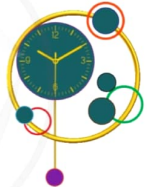
\includegraphics[scale=1]{images/9C5-1-1.png}}
	\loigiai{
	\begin{enumerate}
	\item Cặp đường tròn cắt nhau là vòng tròn màu tím và vòng tròn màu vàng.
	\item Cặp đường tròn tiếp xúc ngoài là vòng tròn màu xanh lá cây và vòng tròn màu xanh.
	\item Cặp đường tròn tiếp xúc trong là vòng tròn màu vàng và vòng tròn của đồng hồ.
	\item Cặp đường tròn không giao nhau là vòng tròn màu xanh và vòng tròn màu đỏ.
	\end{enumerate}
	}
\end{bt}
%%==========Bài 1
\begin{bt} Cho hai điểm $O$ và $O'$ cách nhau một khoảng $5$ cm. Mỗi đường tròn sau đây có vị trí tương đối như thế nào đối với đường tròn $\left(O;3\,\text{cm} \right)$.
	\begin{multicols}{3}
	\begin{listEX}[1]
	\item Đường tròn $\left(O';3\,\text{cm} \right)$;
	\item Đường tròn $\left(O';1\,\text{cm} \right)$;
	\item Đường tròn $\left(O';8\,\text{cm} \right)$.
	\end{listEX}
	\end{multicols}	
	\loigiai{
	\begin{listEX}[1]
	\item 	Đặt $R=3$ cm, $R'=3$ cm ta có $OO'=5 \, \text{cm}<R+R'$. Vậy hai đường tròn đã cho cắt nhau.
	\item 	Đặt $R=3$ cm, $R'=1$ cm ta có $OO'=5 \, \text{cm}>R+R'$. Vậy hai đường tròn đã cho ở ngoài nhau.
	\item 	Đặt $R=3$ cm, $R'=8$ cm ta có $OO'=5 \, \text{cm}=R'-R$. Vậy hai đường tròn đã cho tiếp xúc nhau.
	\end{listEX}
	}
\end{bt}
%%==========Bài 7
\begin{bt}
	Xác định vị trí tương đối của $(O ; R)$ và $(O'; R')$ trong mỗi trường hợp sau
	\begin{listEX} [2]
	\item $OO'=18 $; $R=10$; $R'=6$;
	\item $OO'=2 $; $R=9$; $R'=3$;
	\item $OO'=13 $; $R=8$; $R'=5$;
	\item $OO'=17 $; $R=15$; $R'=4$;
	\end{listEX}
	\loigiai{
	\begin{listEX} [1]
	\item $OO'=18 $; $R=10$; $R'=6$.\\
	Ta có $OO'=18 >R+R'=10+6$ nên hai đường tròn $(O)$ và $(O')$ ngoài nhau.
	\item $OO'=2 $; $R=9$;$R'=3$.\\
	Ta có $OO'=2<R-R'=9-3=6$ nên hai đường tròn $(O)$ và $(O')$ đựng nhau.
	\item $OO'=13 $; $R=8$; $R'=5$.\\
	Ta có $OO'=13=R+R'=8+5$ nên hai đường tròn $(O)$ và $(O')$ tiếp xúc ngoài với nhau.
	\item $OO'=17 $; $R=15$; $R'=4$.\\
	Ta có $R-R'=11<OO'=17<R+R'=19$ nên hai đường tròn $(O)$ và $(O')$ cắt nhau theo hai giao điểm.
	\end{listEX}	
	}
\end{bt}
%%==========Bài 2
\begin{bt} Cho ba điểm $O$, $A$ và $O'$. Với mỗi trường hợp sau, hãy viết hệ thức giữa các độ dài $OO'$, $OA$ và $O'A$ rồi xét xem hai đường tròn $\left(O;OA \right)$ và $\left(O';O'A \right)$ tiếp xúc trong hay tiếp xúc ngoài với nhau; vẽ hình để khẳng định dự đoán của mình.
	\begin{listEX}[3]
	\item $A$ nằm giữa $O$ và $O'$.
	\item $O$ nằm giữa $A$ và $O'$.
	\item $O'$ nằm giữa $A$ và $O$.
	\end{listEX}
	\loigiai{
	\begin{listEX}[1]
	\item Vì điểm $A$ nằm giữa hai điểm $O$ và $O'$ nên $OO'=OA+O'A$ nên hai đường tròn $\left(O;OA \right)$ và $\left(O';O'A \right)$ tiếp xúc ngoài.
	\begin{center}
	\begin{tikzpicture}[scale=0.7, font=\footnotesize, line join=round, line cap=round, >=stealth]
	\def\R{2.5}
	\def\r{1}	
	\path (0,0) coordinate (O)
	(\R,0) coordinate (A)
	(3.5,0) coordinate (O')
	($(O') + (0:\r)$) coordinate (A');
	\path[name path = dtO](O) let \p1=($(O)-(A)$) in circle ({veclen(\x1,\y1)});
	\path[name path = dtO'](O') let \p1=($(O')-(A')$) in circle ({veclen(\x1,\y1)});
	\path[name intersections = {of = dtO and dtO', by ={M}}];
	\draw (O)--(O');
	\pgfresetboundingbox
	\draw (O) let \p1=($(O)-(A)$) in circle ({veclen(\x1,\y1)});
	\draw[blue ] (O') let \p1=($(O')-(A')$) in circle ({veclen(\x1,\y1)});
	\foreach \x/\g in {O/-90,O'/-90,A/160}\draw[fill=black](\x) circle (.05) + (\g:.4) node{$\x$};
	\end{tikzpicture} \end{center}
	\item Vì điểm $O$ nằm giữa hai điểm $A$ và $O'$ nên $OO'=O'A-OA$ nên hai đường tròn $\left(O;OA \right)$ và $\left(O';O'A \right)$ tiếp xúc trong.
	\begin{center}
	\begin{tikzpicture}[scale=0.7, font=\footnotesize, line join=round, line cap=round, >=stealth]
	\def\R{2.5}
	\def\r{1}	
	\path (0,0) coordinate (O')
	(\R,0) coordinate (A)
	(1.5,0) coordinate (O)
	($(O) + (0:\r)$) coordinate (A');
	\path[name path = dtO'](O') let \p1=($(O')-(A)$) in circle ({veclen(\x1,\y1)});
	\path[name path = dtO](O) let \p1=($(O)-(A')$) in circle ({veclen(\x1,\y1)});
	%\path[name intersections = {of = dtO and dtO', by ={M}}];
	\draw (A)--(O');
	\pgfresetboundingbox
	\draw (O') let \p1=($(O')-(A)$) in circle ({veclen(\x1,\y1)});
	\draw[blue ] (O) let \p1=($(O)-(A')$) in circle ({veclen(\x1,\y1)});
	\foreach \x/\g in {O/-90,O'/-90,A/0}\draw[fill=black](\x) circle (.05) + (\g:.4) node{$\x$};
	\end{tikzpicture} 
	\end{center}
	\item Vì điểm $O'$ nằm giữa hai điểm $A$ và $O$ nên $OO'=OA-O'A$ nên hai đường tròn $\left(O;OA \right)$ và $\left(O';O'A \right)$ tiếp xúc trong.
	\begin{center}
	\begin{tikzpicture}[scale=0.7, font=\footnotesize, line join=round, line cap=round, >=stealth]
	\def\R{2.5}
	\def\r{1}	
	\path (0,0) coordinate (O)
	(\R,0) coordinate (A)
	(1.5,0) coordinate (O')
	($(O') + (0:\r)$) coordinate (A');
	\path[name path = dtO](O) let \p1=($(O)-(A)$) in circle ({veclen(\x1,\y1)});
	\path[name path = dtO'](O') let \p1=($(O')-(A')$) in circle ({veclen(\x1,\y1)});
	%\path[name intersections = {of = dtO and dtO', by ={M}}];
	\draw (O)--(A);
	\pgfresetboundingbox
	\draw (O) let \p1=($(O)-(A)$) in circle ({veclen(\x1,\y1)});
	\draw[blue ] (O') let \p1=($(O')-(A')$) in circle ({veclen(\x1,\y1)});
	\foreach \x/\g in {O/-90,O'/-90,A/0}\draw[fill=black](\x) circle (.05) + (\g:.4) node{$\x$};
	\end{tikzpicture} \end{center}
	\end{listEX}
	}
\end{bt}
%%==========Bài 3
\begin{bt} Cho hai đường tròn $\left(O\right)$ và $\left(O'\right)$ tiếp xúc ngoài với nhau tại $A$. Một đường thẳng qua $A$ cắt $\left(O\right)$ tại $B$ và cắt $\left(O'\right)$ tại $C$. Chứng minhh rằng $OB \parallel O'C$.
	\loigiai{
	\immini{
	Xét tam giác $OBA$ cân tại $O$ nên $\widehat{OBA}=\widehat{OAB}$.\\
	Xét tam giác $O'CA$ cân tại $O'$ nên $\widehat{O'CA}=\widehat{O'AC}$.\\
	Mà $\widehat{OAB}=\widehat{O'AC}$ (hai góc đối đỉnh) nên $\widehat{OBA}=\widehat{O'CA}$. \\
	Mà hai góc này lại ở vị trí so le trong nên suy ra $OB \parallel O'C$.
	}{
	\begin{tikzpicture}[scale=1, font=\footnotesize, line join=round, line cap=round, >=stealth]
	\def\R{2}
	\def\r{1}	
	\path (0,0) coordinate (O)
	(\R,0) coordinate (A)
	(3.5,0) coordinate (O')
	($(O') + (0:\r)$) coordinate (A')
	($(O) + (70:\R)$) coordinate (B)
	($(O') + (-110:\r)$) coordinate (C);
	\path[name path = dtO](O) let \p1=($(O)-(A)$) in circle ({veclen(\x1,\y1)});
	\path[name path = dtO'](O') let \p1=($(O')-(A')$) in circle ({veclen(\x1,\y1)});
	\path[name intersections = {of = dtO and dtO', by ={M}}];
	\draw (O)--(O') (C)--(O') (O)--(B) (B)--(C);
	\pgfresetboundingbox
	\draw (O) let \p1=($(O)-(A)$) in circle ({veclen(\x1,\y1)});
	\draw[blue ] (O') let \p1=($(O')-(A')$) in circle ({veclen(\x1,\y1)});
	\foreach \x/\g in {O/-90,O'/90,A/160,B/90,C/-90}\draw[fill=black](\x) circle (.05) + (\g:.4) node{$\x$};
	\end{tikzpicture}
	}
	}
\end{bt}
%%==========Bài 5
\begin{bt}
	Cho hai đường tròn $(O ; 2 \mathrm{~cm})$ và $(A ; 2 \mathrm{~cm})$ cắt nhau tại $C$, $D$, điểm $A$ nằm trên đường tròn tâm $O$.
	\begin{listEX} [1]
	\item Vẽ đường tròn $(C ; 2 \mathrm{~cm})$.
	\item Đường tròn $(C ; 2 \mathrm{~cm})$ có đi qua hai điểm $O$ và $A$ không? Vì sao?
	\end{listEX}
	\loigiai{
	\immini{
	\begin{listEX} [1]
	\item Vẽ đường tròn $(C ; 2 \mathrm{~cm})$ (Hình bên).
	\item Đường tròn $(O ; 2 )$ và $(A ; 2 )$ cắt nhau tại $C$, $D$, điểm $A$ nằm trên đường tròn tâm $O$ nên $OC=OD=2$ cm, $AC=AD=2$ cm.\\
	Suy ra $CO=CA=2$ cm. Do đó đường tròn $(C ; 2 \mathrm{~cm})$ đi qua hai điểm $O$ và $A$.
	\end{listEX}}{\begin{tikzpicture}[scale=0.7]
	\def\r{2}
	\def\v{2}
	\def\u{2}
	\path
	(0:0) coordinate (O)
	(0:\r) coordinate (A)
	;
	\draw[black] (O) circle (\r);
	\draw[black] (A) circle (\v);
	\path[name path=c1] (O) circle (\r);
	\path[name path=c2] (A) circle (\v);
	\path[name intersections={of=c1 and c2,by={C,D}}]; 
	\draw[black] (C) circle (\u);
	\foreach \x/\g in {D/-90,O/180,A/0,C/90}
	\draw [fill= white] (\x) circle (.05)+(\g:.5) node{$\x$};
	\end{tikzpicture}}
	}
\end{bt}
%%==========Bài 6
\begin{bt}
	Cho hai đường tròn $(A ; 6 \mathrm{~cm})$ và $(B ; 4 \mathrm{~cm})$ cắt nhau tại $C$ và $D$, $AB=8 \mathrm{~cm}$. Gọi $K$, $I$ lần lượt là giao điểm của hai đường tròn đâ cho với đoạn thẳng $AB$.
	\begin{listEX} [1]
	\item Tính độ dài của các đoạn thẳng $CA$, $CB$, $DA$ và $DB$.
	\item Điểm $I$ có phải là trung điểm của đoạn thẳng $AB$ không?
	\item Tính độ dài của đoạn thẳng $IK$.
	\end{listEX}
	\loigiai{
	\immini{\begin{listEX} [1]
	\item Hai đường tròn $(A ; 6 \mathrm{~cm})$ và $(B ; 4 \mathrm{~cm})$ cắt nhau tại $C$ và $D$ nên $AC=AD=6$ cm, $BC=BD=4$ cm.
	\item $AB=8$ cm. $BC=BD=BI=4$ cm. Suy ra $AI=AB-IB= 8-4=4$ cm. Điểm $I$ là trung điểm của đoạn thẳng $AB$.
	\item Ta có $AK=AC=6$ cm nên $IK=AK-AI=6-4=2$ cm.
	\end{listEX}}{	\begin{tikzpicture}[scale=0.35]
	\def\r{6}
	\def\v{4}
	\path
	(0:0) coordinate (A)
	(0:8) coordinate (B)
	(0:4) coordinate (I)
	(0:6) coordinate (K)
	;
	\draw[black] (A) circle (\r);
	\draw[black] (B) circle (\v);
	\path[name path=c1] (A) circle (\r);
	\path[name path=c2] (B) circle (\v);
	\path[name intersections={of=c1 and c2,by={C,D}}]; 
	\draw (A)--(C)--(B)--(A)--(D)--(B);
	\foreach \x/\g in {D/-90,B/0,A/180,C/80,I/135,K/45}
	\draw [fill= white] (\x) circle (.05)+(\g:.5) node{$\x$};
	\end{tikzpicture}}
	}
\end{bt}
%%%%
\begin{bt}%[9H2B8]
	Cho $I$ là trung điểm của đoạn thẳng $AB$. Xác định vị trí tương đối của hai đường tròn ($I$; $IA$) và ($B$; $BA$).
	\loigiai
	{
	\immini
	{Vì $I$ là trung điểm của đoạn thẳng $AB$ nên ta có $A$, $I$, $B$ thẳng hàng và $BI=BA=IA$, từ đó suy ra ($I$; $IA$) tiếp xúc trong với ($B$; $BA$) tại $A$.}
	{\begin{tikzpicture}[line join = round, line cap = round,>=stealth,scale=1]
	\tkzDefPoints{0/0/A}
	\tkzDefPoints{1/0/I}
	\tkzDefPoints{2/0/B}
	\pgfresetboundingbox
	\tkzDrawCircle[radius,black](I,A)
	\tkzDrawCircle[radius,black](B,A)
	\tkzDrawPoints[fill=black](B,I,A)
	\tkzDrawSegments(B,A)
	\tkzLabelPoints[left](A)
	\tkzLabelPoints[below](I)
	\tkzLabelPoints[right](B)
	\end{tikzpicture}	}
	}
\end{bt}
\begin{bt}%[9H2B8]
	Cho hai đường tròn ($O$; $8$ cm) và ($O'$; $3$ cm). Kẻ tiếp tuyến chung ngoài $AB$ (với $A$ thuộc $(O)$; $B$ thuộc $(O')$). TÍnh độ dài đoạn $AB$ nếu $OO' =13$ cm.
	\loigiai
	{
	\immini
	{Kẻ $O'H\perp OA$ tại $H$ $\Rightarrow $ tứ giác $ABO'H$ là hình chữ nhật \\
	$\Rightarrow AB=O'H$, $AH=O'B=3.$\\
	Áp dụng định lí Py-ta-go vào $\triangle HOO'$ ta có
	$$ O'H=\sqrt{OO'^2-OH^2}=\sqrt{13^2-(8-3)^2}=12.$$
	Vậy $AB=12$ cm.}
	{\begin{tikzpicture}[line join = round, line cap = round,>=stealth,scale=0.4]
	\tkzDefPoints{0/0/O}
	\tkzDefPoints{4.5/0/Q}
	\tkzDefPoints{8.5/0/O'}
	\tkzDefPoints{6.5/0/P}
	\pgfresetboundingbox
	\tkzDrawPoints[fill=black](O,O')
	\tkzDrawCircle[radius,black](O,Q)
	\tkzDrawCircle[radius,black](O',P)
	\tkzInterLC[R](O,O')(O,2.5cm) \tkzGetPoints{}{g}
	\tkzDefTangent[from=O'](O,g) \tkzGetPoints{b}{a}
	\tkzInterLC[R](O,a)(O,4.5 cm) \tkzGetPoints{}{A}
	\coordinate (B) at ($(A)+(O')-(a)$);
	\tkzDefPointBy[projection = onto O--A](O') \tkzGetPoint{H}
	\tkzDrawSegments(O,O' O,A O',B A,B O',H)
	\tkzDrawPoints[fill=black](O,O',A,B,H)
	\tkzMarkRightAngles[size=0.2](O',B,A O,A,B)
	\tkzLabelPoints[above](A,B)
	\tkzLabelPoints[left](O,H)
	\tkzLabelPoints[below left](O')
	\path (O)--(H) node[above,midway,sloped]{$5$};
	\path (O)--(O') node[above,midway,sloped]{$13$};
	\path (H)--(A) node[above,midway,sloped]{$3$};
	\end{tikzpicture}}
	}
\end{bt}
\begin{bt}%[9H2B8]
	Cho ba điểm $A$, $B$, $C$ thẳng hàng theo thứ tự đó và dựng các đường tròn đường kính $AB$, $BC$. Từ $A$ vẽ tiếp tuyến $AD$ với đường tròn đường kính $BC$ ($D$ là tiếp điểm), tiếp tuyến $AD$ cắt đường tròn đường kính $AB$ tại $E$ ($E \ne A$). Chứng minh rằng tia $BD$ là tia phân giác của góc $EBC$.
	\loigiai
	{
	Kẻ tiếp tuyến chung $Bx$; $Bx$ cắt $DE$ tại $F$ như hình vẽ.
	\begin{center}
	\begin{tikzpicture}[line join = round, line cap = round,>=stealth,scale=1]
	\tkzDefPoints{0/0/A}
	\tkzDefPoints{2/0/B}
	\tkzDefPoints{6/0/C}
	\coordinate (I) at ($(B)!0.5!(C)$);
	\coordinate (M) at ($(A)!0.5!(B)$);
	\tkzDefTangent[from=A](I,C) \tkzGetPoints{D}{d}
	\tkzInterLC(A,D)(M,A) \tkzGetPoints{E}{}
	\tkzDefPointWith[orthogonal,K=1.3](B,I) \tkzGetPoint{x}
	\tkzInterLL(x,B)(E,D) \tkzGetPoint{F}
	\pgfresetboundingbox
	\tkzDrawPoints[fill=black](A,B,C,D,E,F)
	\tkzDrawCircle[radius,black](I,C)
	\tkzDrawCircle[radius,black](M,A)
	\tkzDrawSegments(B,E A,D A,C B,x)
	\tkzDrawSegments[dashed](D,I)
	\tkzMarkRightAngles[size=0.2](A,E,B E,D,I F,B,C)
	\tkzLabelPoints[above](D,E)
	\tkzLabelPoints[left](A,x)
	\tkzLabelPoints[right](C)
	\tkzLabelPoints[below left](B)
	\tkzLabelPoints[above right](F)
	\end{tikzpicture}
	\end{center}
	\begin{itemize}
	\item Vì $E$ thuộc đường tròn đường kính $AB$ nên $\widehat{AEB}=90^\circ.$ $\hfill$ $(1)$
	\item Vì $BF$ là tiếp tuyến của đường tròn đường kính $AB$ tại $B$ nên $BF \perp AB$ tại $B$ hay $\widehat{ABF}=90^\circ.$$\hfill$ $(2)$\\
	Từ $(1)$ và $(2)$ suy ra $\widehat{FAB}=\widehat{FBE}$ (cùng phụ với $\widehat{AFB}$) hay $\widehat{DAB}=\widehat{EBF}$.
	\item Vì $DF$, $FB$ là hai tiếp tuyến của đường tròn đường kính $BC$ nên $FD=FB$ suy ra $\triangle FDB$ cân tại $F \Rightarrow\; \widehat{FDB}=\widehat{FBD}.$\\
	Do đó $\widehat{EBD}=\widehat{EBF}+\widehat{FBD}=\widehat{DAB}+\widehat{FDB}.$\\
	Mà $\widehat{DBC}=\widehat{FDB}+\widehat{DAB}$ (tính chất góc ngoài của $\triangle ABD$) nên $\widehat{EBD}=\widehat{DBC},$ do đó $BD$ là tia phân giác của $\widehat{EBC}$. 
	\end{itemize}
	}
\end{bt}
\begin{bt}%[9H2B8]
	Cho hình vuông $ABCD$, lấy điểm $M$ bất kì trên đường chéo $BD$ ($M\ne B$; $M \ne D$). Vẽ đường tròn $(O)$ qua $M$ và tiếp xúc với $AB$ tại $B$, vẽ đường tròn $(O')$ qua $M$ và tiếp xúc với $AD$ tại $D$. Hai đường tròn $(O)$ và $(O')$ cắt nhau tại điểm thứ hai $N$ (với $N\ne M$).
	\begin{enumerate}
	\item Chứng minh rằng $O'N$ là tiếp tuyến của đường tròn $(O)$ và $ON$ là tiếp tuyến của đường tròn $(O')$.
	\item Khi $M$ di động trên $BD$, tìm giá trị nhỏ nhất của độ dài đoạn $OO'$ theo cạnh hình vuông $ABCD$.
	\end{enumerate}
	\loigiai
	{
	\begin{enumerate}
	\item Vì $AB$ là tiếp tuyến của đường tròn $(O)$ nên tâm $O$ của $(O)$ phải nằm trên đường thẳng vuông góc với $AB$ tại $B$. Mà $BC \perp AB$ tại $B$ (vì $ABCD$ là hình vuông) nên $O$ thuộc $BC$.
	\immini{
	Vì $M$ thuộc $(O)$ nên $ON=OM \Rightarrow\; \triangle OBM$ cân tại $O$ $\Rightarrow\; \widehat{OMB}=\widehat{OBM}=\widehat{CBD}=45^\circ \Rightarrow\; \triangle OBM$ vuông cân tại $O$\\
	$\Rightarrow\; \widehat{BOM}=90^\circ$ hay $\widehat{COM}=90^\circ.$\\
	Tương tự ta có $\widehat{CO'M}=90^\circ.$\\
	Từ đó suy ra tứ giác $COC'M$ là hình chữ nhật $\Rightarrow \; \widehat{OMO'}=90^\circ.$\\
	Vì $\triangle OMO' = \triangle ONO'$ (c.c.c) nên $\widehat{ONO'}=\widehat{OMO'}=90^\circ$\\
	$\Rightarrow ON$ là tiếp tuyến của $(O')$ và $O'N$ là tiếp tuyến của $(O)$.
	\item Vì tứ giác $OCO'M$ là hình chữ nhật nên $OO'=CM$. \\
	$OO'$ nhỏ nhất $\Leftrightarrow\; CM$ nhỏ nhất $\Leftrightarrow \; CM \perp BD$ tại $M$ $\Leftrightarrow M$ là giao điểm của $AC$ và $BD$.\\
	Do đó $OO'_{\text{min}}=\dfrac{1}{2}BD=\dfrac{a\sqrt{2}}{2}$ (với $AB=BC=CD=DA=a$) khi $M$ là tâm của hình vuông $ABCD$. 
	}
	{\begin{tikzpicture}[line join = round, line cap = round,>=stealth,font=\footnotesize,scale=0.85]
	\tkzDefPoints{0/0/A}
	\coordinate (B) at ($(A)+(4,0)$);
	\tkzDefSquare(B,A) \tkzGetPoints{D}{C}
	\coordinate (M) at ($(B)!0.3!(D)$);
	\tkzDefPointBy[projection = onto B--C](M) \tkzGetPoint{O}
	\tkzDefPointBy[projection = onto C--D](M) \tkzGetPoint{O'}
	\tkzInterCC(O,M)(O',M) \tkzGetPoints{N}{}
	\coordinate (x) at ($(O)!2!(N)$);
	\coordinate (y) at ($(O')!2!(N)$);
	\tkzInterLC(B,C)(O',M) \tkzGetPoints{}{Q}
	\pgfresetboundingbox
	\tkzDrawCircle[radius](O,M)
	\tkzDrawCircle[radius](O',M)
	\tkzDrawPolygon(A,B,C,D)
	\tkzDrawSegments(B,D M,O M,O' O,x O',y O',Q)
	\tkzDrawPoints[fill=black](A,B,D,C,M,N,Q)
	\tkzLabelPoints[above](A,B)
	\tkzLabelPoints[below](C,O')
	\tkzLabelPoints[above left](M)
	\tkzLabelPoints[right](N)
	\tkzLabelPoints[above right](O)
	\tkzLabelPoints[left](D)
	\tkzMarkRightAngles[size=0.2](A,B,O B,O,M O,C,O' O',D,A)
	\tkzMarkSegments[mark=|](A,B A,D)
	\end{tikzpicture}}
	\end{enumerate}
	}
\end{bt}
\begin{bt}%[9H2B8]
	Cho ($O$; $4$ cm), ($O'$; $2$ cm) và $OO'=9$ cm. Dựng tiếp tuyến chung trong của $(O)$ và $(O')$.
	\loigiai
	{
	Các phần phân tích, chứng minh, biện luận dành cho bạn đọc.
	\begin{center}
	\begin{tikzpicture}[line join = round, line cap = round,>=stealth,font=\footnotesize,scale=0.6]
	\tkzDefPoints{0/0/O}
	\tkzDefPoints{6/0/I}
	\tkzDefPoints{9/0/O'}
	\tkzDefPoints{4/0/P}
	\tkzDefPoints{7/0/Q}
	\coordinate (R) at ($(O)!0.5!(I)$);
	\tkzInterCC(O,P)(R,O) \tkzGetPoints{A}{A'}
	\tkzDefPointBy[projection = onto A--I](O') \tkzGetPoint{B}
	\tkzDefPointBy[projection = onto A'--I](O') \tkzGetPoint{B'}
	\coordinate (T) at ($(I)!1.5!(A)$);
	\coordinate (K) at ($(I)!1.5!(B)$);
	\coordinate (T') at ($(I)!1.5!(A')$);
	\coordinate (K') at ($(I)!1.5!(B')$);
	\pgfresetboundingbox
	\tkzDrawPoints[fill=black](A,B,I,O,O',A')
	\tkzDrawCircle[radius,black](O,P)
	\tkzDrawCircle[radius,black](O',Q)
	\tkzDrawCircle[dashed](R,O)
	\tkzDrawSegments(O,O' O,A O',B T,K)
	\tkzDrawSegments[dashed](T',K')
	\tkzMarkRightAngles[size=0.2](O,A,I O',B,I)
	%\tkzLabelPoints[below right](I)
	\tkzLabelPoints[left](O)
	\tkzLabelPoints[right](O')
	\tkzLabelPoints[below left](B)
	\tkzLabelPoints[above right](A,I)
	\path (O)--(A) node[above,midway,sloped]{$4$};
	\path (O')--(B) node[above,midway,sloped]{$2$};
	\end{tikzpicture}
	\end{center}
	- Dựng điểm $I$ là điểm chia trong của đoạn $OO'$ với tỉ số $\dfrac{R}{R'}=\dfrac{2}{1},$ tức là $I$ nằm trong đoạn $OO'$ và $\dfrac{IO}{IO'}=\dfrac{R}{R'}=\dfrac{2}{1}$ hay $\dfrac{IO}{IO'+IO}=\dfrac{2}{2+1} \Leftrightarrow \; \dfrac{IO}{9}=\dfrac{2}{3} \Leftrightarrow\; IO=6$ (cm)\\
	- Dựng đường tròn đường kính $IO$, đường tròn này cắt đường tròn $(O)$ tại $A$ và $A'$.\\
	- Dựng đường thẳng $AI$ và $A'I$ là hai tiếp tuyến chung trong cần dựng.
	}
\end{bt}
\begin{bt}%[9H2B8]
	Cho đường thẳng $d$. Lấy điểm $O$ thuộc $d$, vẽ hai nửa đường tròn ($O$; $r$) và ($O$; $R$) (với $0<r<R$) trên cùng một nửa mặt phẳng bờ $d$. Chứng minh: điều kiện cần và đủ để có hai điểm $A$, $D$ thuộc ($O$; $r$) và hai điểm $B$, $C$ thuộc ($O$; $R$) sao cho $ABCD$ là một hình vuông là $r<R \leq r\left( \sqrt{2}+1 \right).$
	\loigiai
	{
	\immini{Kẻ $Ox \perp d$ tại $O$; $Ox$ cắt $BC$ tại $H$, cắt $AD$ tại $K$.\\
	Ta có
	\begin{align*}
	OK=\sqrt{r^2-\frac{a^2}{4}}\\
	OH=\sqrt{R^2-\frac{a^2}{4}}
	\end{align*}
	(với $a=AB=BC=CD=DA$).}
	{\begin{tikzpicture}[line join = round, line cap = round, >=stealth, font=\footnotesize, scale=1.2]
	\tikzset{label style/.style={font=\footnotesize}}
	\def\R{3} \def\r{1.5}
	\coordinate[label={below right}:{$O$}] (O) at (0,0);
	\coordinate (x) at ($(O)+(\R,0)$);
	\coordinate (x') at ($(O)+(-\R,0)$);
	\coordinate (y) at ($(O)+(\r,0)$);
	\coordinate (y') at ($(O)+(-\r,0)$);
	\draw (x) arc (0:180:\R cm);
	\draw (y) arc (0:180:\r cm);
	\tkzDrawLine[add = 0.1 and 0](x,x')
	\coordinate[label={right}:{$D$}] (D) at ($(O)+(60:\r cm)$);
	\coordinate[label={left}:{$A$}] (A) at ($(O)+(120:\r cm)$);
	\coordinate[label={above right}:{$C$}] (C) at ($(O)+(75:\R cm)$);
	\coordinate[label={above left}:{$B$}] (B) at ($(O)+(105:\R cm)$);
	\coordinate[label={below right}:{$H$}] (H) at ($(B)!0.5!(C)$);
	\coordinate[label={below right}:{$K$}] (K) at ($(A)!0.5!(D)$);
	\tkzDrawLine[add = 0 and 0.3](O,H)
	\draw[dashed] (O)--(B);
	\draw (A)--(B)--(C)--(D)--cycle;
	\draw (O)--(A);
	\tkzLabelLine[above right, pos=1.1](x',x){$d$}
	\tkzLabelLine[right, pos=1.3](O,H){$x$}
	\tkzLabelSegment[left](O,A){$r$}
	\tkzLabelSegment[right, pos=0.7](O,B){$R$}
	\tkzLabelSegment[left](A,B){$a$}
	\tkzMarkRightAngles[size=0.15](O,H,B O,K,A D,C,B C,D,A D,A,B A,B,C)
	\tkzDrawPoints[fill=black](O,D,A,B,C,H,K)
	\end{tikzpicture}}
	Vì $OH=OK+KH$ nên $\sqrt{R^2-\dfrac{a^2}{4}}=\sqrt{r^2-\dfrac{a^2}{4}}+a$\\
	$\Rightarrow 2a^4-2(R^2+r^2)a^2+(R^2-r^2)^2=0$\\
	$\Leftrightarrow \left[a^2-\dfrac{1}{2} (R^2-r^2)\right]^2=4R^2r^2-(R^2-r^2)^2.$$\hfill$$(*)$\\
	Do đó để tồn tại hình vuông $ABCD$ thì phải tồn tại $a$ $\Rightarrow (*)$ phải có nghĩa hay 
	\begin{align*}
	&4R^2r^2-(R^2-r^2)^2 \geq 0\\
	\Leftrightarrow\; &4R^2r^2 \geq (R^2-r^2)^2\\
	\Leftrightarrow\; &\sqrt{4R^2r^2} \geq \sqrt{(R^2-r^2)^2}\\
	\Leftrightarrow\; &2Rr \geq R^2-r^2 (\text{vì} R>r>0)\\
	\Leftrightarrow\; &r^2 \geq R^2-2Rr\\
	\Leftrightarrow\; &2r^2 \geq (R-r)^2\\
	\Leftrightarrow\; &\sqrt{2}r \geq R-r\\
	\Leftrightarrow\; &(1+\sqrt{2})r \geq R.
	\end{align*}
	Kết hợp với điều kiện $R>r$, ta có $r<R \leq (1+\sqrt{2})r.$
	}
\end{bt}